\documentclass[aspectratio=169]{beamer}
% \usetheme{Madrid}

\usefonttheme{serif}
\setbeamercolor{normal text}{fg=black}

% Make all structural text black (titles, sections, etc.)
\setbeamercolor{structure}{fg=black}

% Frame titles (top title)
\setbeamercolor{frametitle}{fg=black}

% Figure caption ("Figure:")
\setbeamercolor{caption name}{fg=black}
\setbeamercolor{caption}{fg=black}

% Section titles in footer/header
\setbeamercolor{section in head/foot}{fg=black}

% Just in case
\setbeamercolor{title}{fg=black}


% --- Theme setup (minimal) ---
\usetheme{default}
\useoutertheme{default}
\useinnertheme{default}

% Remove navigation symbols
\setbeamertemplate{navigation symbols}{}

% Define your red
% \definecolor{myred}{RGB}{225,120,120}
\definecolor{myred}{RGB}{115,0,10}


\usepackage{color} % color added for editing
\newcommand{\bl}[1]{\textcolor[rgb]{0.00,0.00,1.00}{#1}}
\newcommand{\gr}[1]{\textcolor[rgb]{0.00,0.50,0.00}{#1}}
\newcommand{\rd}[1]{\textcolor[rgb]{0.75,0.00,0.00}{#1}}
\newcommand{\tl}[1]{\textcolor[rgb]{0,0.6,0.60}{#1}}

\usepackage{booktabs}
\usepackage{bm}
\usepackage{mdframed}
\usepackage{xcolor}

% --- Custom footline ---
\setbeamertemplate{footline}{
\leavevmode

% Thin red line (moved to TOP)
\begin{beamercolorbox}[wd=\paperwidth,ht=0.1ex]{}
\color{myred}\rule{\paperwidth}{0.1ex}
\end{beamercolorbox}

\hbox{
\begin{beamercolorbox}[wd=\paperwidth,ht=2.5ex,dp=1ex]{}
\hspace{1em}
\insertsection
\hfill
\insertframenumber{} / \inserttotalframenumber
\hspace{1em}
\end{beamercolorbox}
}
}

% Remove headline entirely
\setbeamertemplate{headline}{}

% Optional: clean fonts
\setbeamerfont{footline}{size=\small}







\title{Chapter~2:~Regression}
\author{Austin R.J. Downey}
\date{}

\begin{document}

\section{Machine Learning for Engineering Problem Solving}
\frame{\titlepage}


\section{Chapter~2~Regression}

%------------------------------------------------
\begin{frame}{Regression}
	\centering
	
\includegraphics[width=0.65\textwidth]{../figures/polynomial_regression_3}
	\vspace{0.3em}
	\small \\
	
	Regression models the relationship between an input variable $x$ (data) and an output variable $y$ (target). The goal is to learn a function that predicts $y$ from $x$.
\end{frame}

%------------------------------------------------

\begin{frame}{Regression Approaches}
	\small
	In this chapter, we examine Linear Regression and two ways to estimate parameters:
	
	\begin{itemize}
		\item \textbf{Closed-form solution:} Solve directly for parameters by minimizing the cost function.
		\item \textbf{Gradient Descent:} Iteratively update parameters to reduce error.
	\end{itemize}
	
	\vspace{0.5em}
	
	Gradient Descent variants:
	\begin{itemize}
		\item Batch Gradient Descent
		\item Stochastic Gradient Descent
		\item Mini-batch Gradient Descent
	\end{itemize}
	
	\vspace{0.5em}
	
	Closed-form gives an exact solution immediately, while Gradient Descent converges through successive updates.
\end{frame}

%------------------------------------------------


\begin{frame}{Data: Ames Housing Dataset}
	\begin{columns}
		\column{0.45\textwidth}
		\small
		The Ames housing dataset contains:
		\begin{itemize}
			\item 2,930 home sales
			\item Data from 2006–2010
			\item Multiple feature types
		\end{itemize}
		\column{0.55\textwidth}
		\centering
		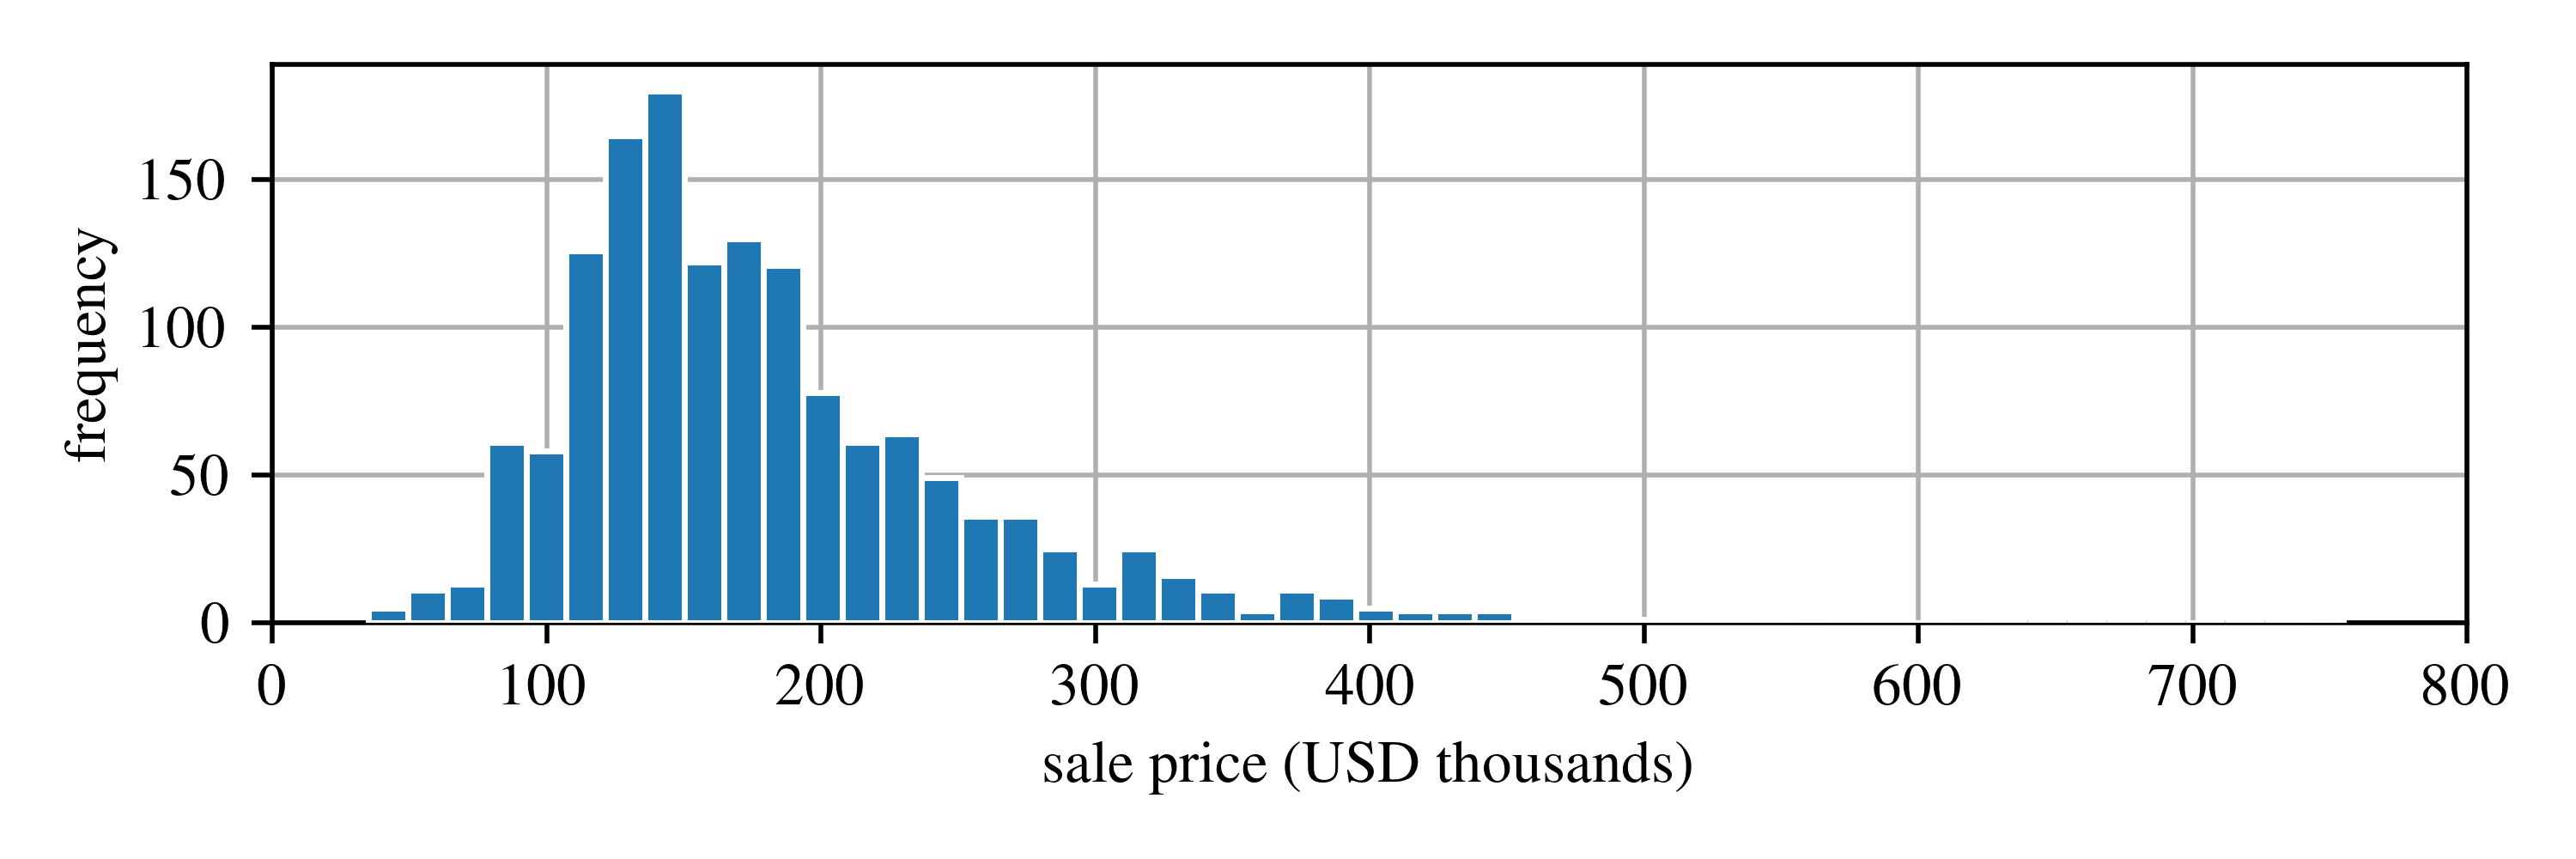
\includegraphics[width=\textwidth]{../figures/Ames_histogram}
		\vspace{0.3em}
		{\small Histogram of sale prices.}
	\end{columns}
\end{frame}

%------------------------------------------------

\begin{frame}{Data: Ames Housing Dataset Feature Correlations}
	\begin{columns}
		\column{0.45\textwidth}
		\small
		Feature relationships:
		\begin{itemize}
			\item Shows correlations between inputs
			\item Helps identify important variables
			\item Useful for feature selection
		\end{itemize}
		\column{0.55\textwidth}
		\centering
		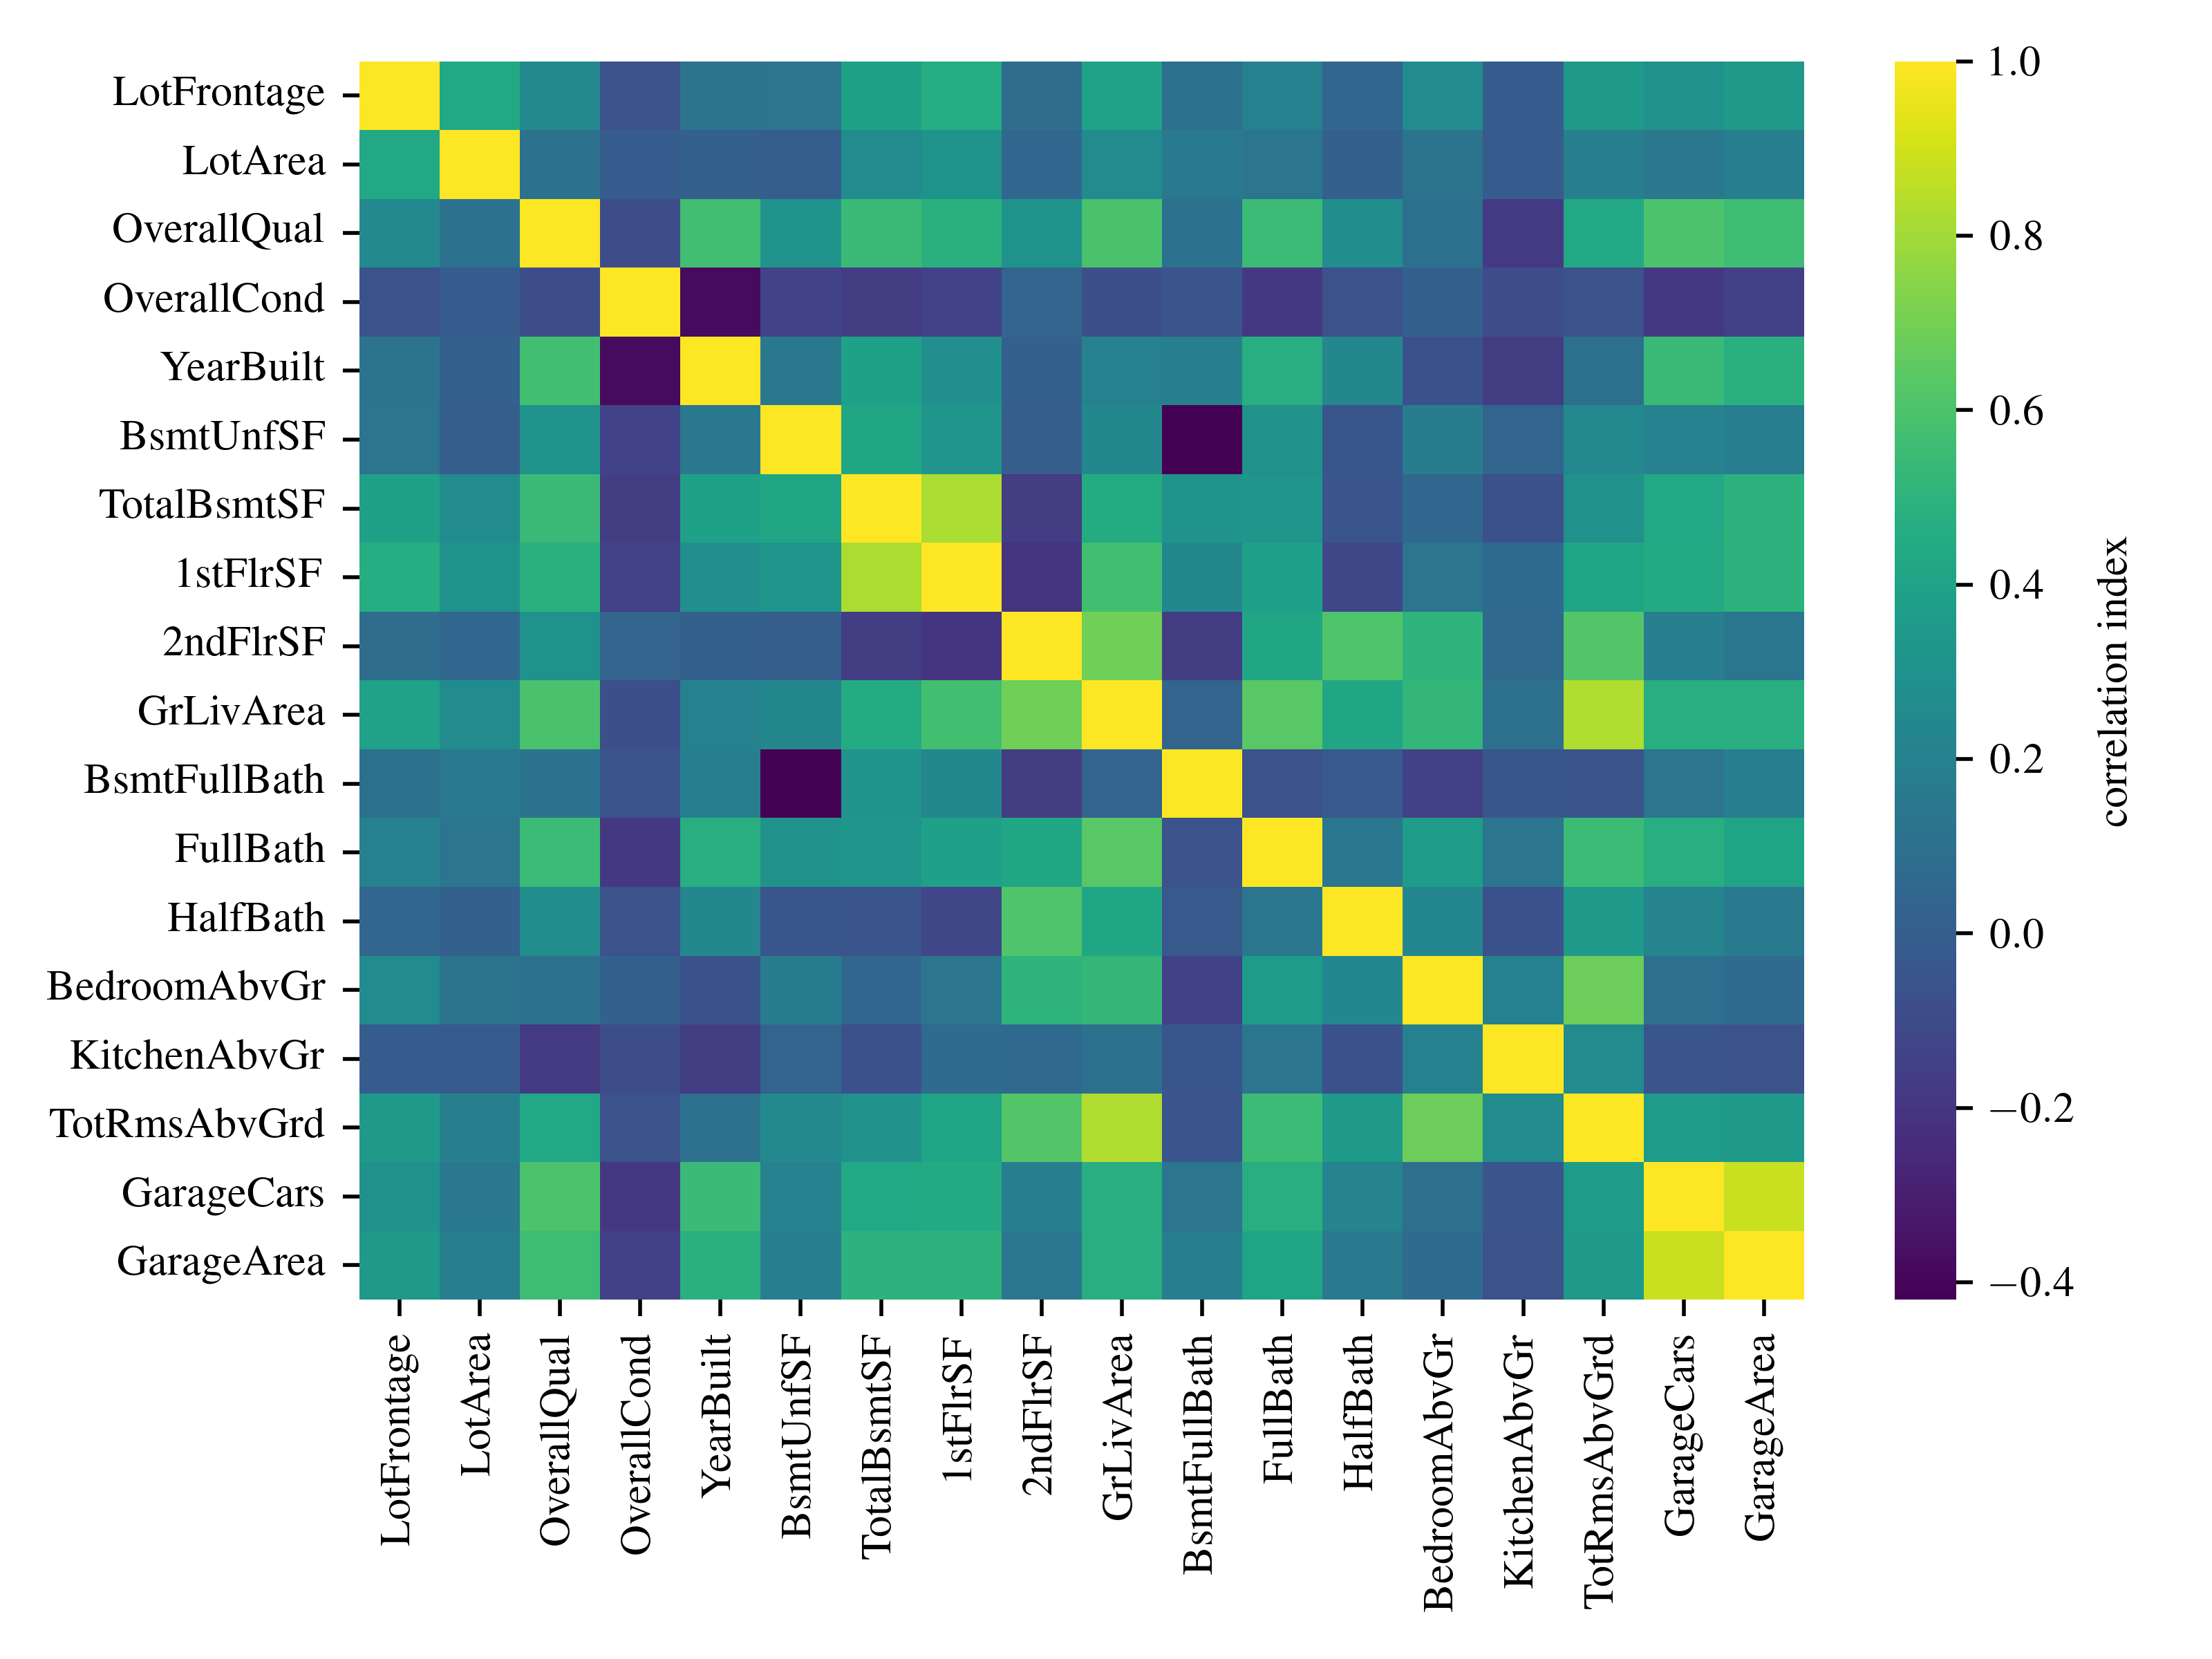
\includegraphics[width=\textwidth]{../figures/Ames_housing_correlation_matirx}
		\vspace{0.3em}
		{\small Correlation matrix of features.}
		\end{columns}
\end{frame}

%------------------------------------------------

\begin{frame}{Ames Housing Example}
	\begin{columns}
		\column{0.48\textwidth}
		\small
		We want to predict house price using the Ames dataset.
				\begin{itemize}
			\item Input: above-ground living area
			\item Target: housing price
			\item Goal: find a linear relationship between them
		\end{itemize}
		\column{0.52\textwidth}
		\centering
		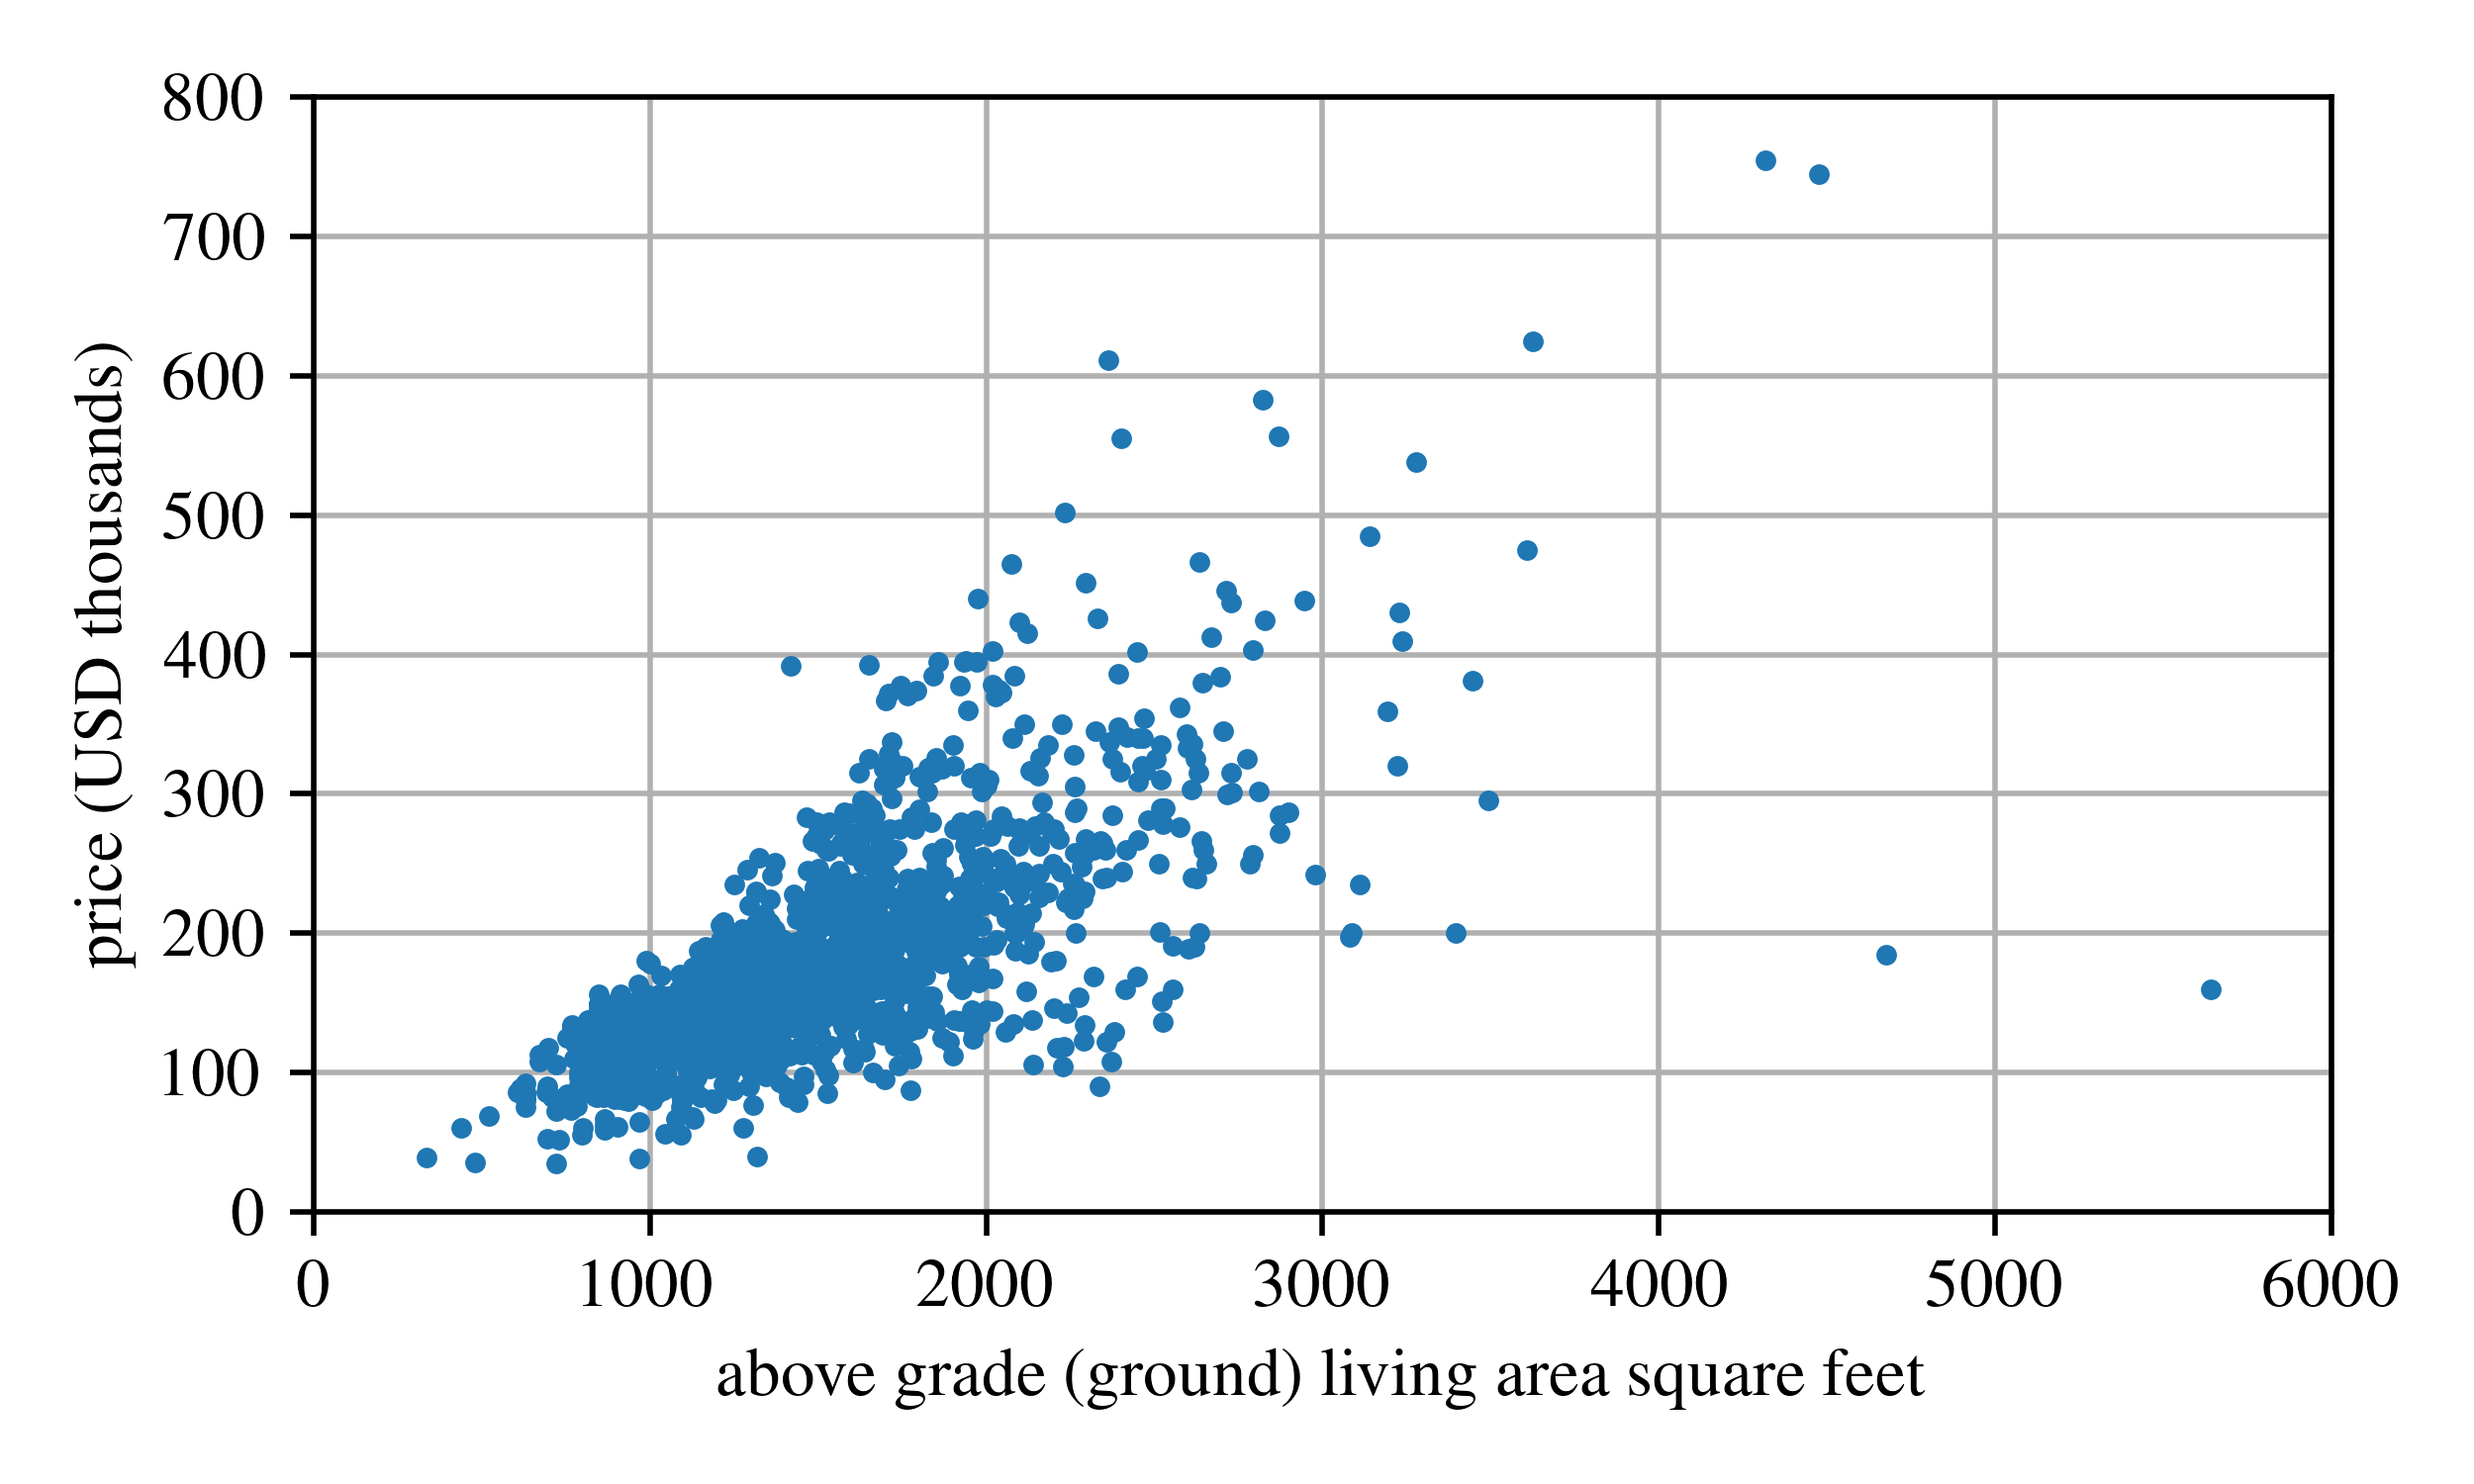
\includegraphics[width=\textwidth]{../figures/Ames_simple_linear_regression_model_1.png}
		\vspace{0.3em}
		{\small Ames housing data.}
		\end{columns}
\end{frame}

%------------------------------------------------
\section{2.1~Linear Regression}

\begin{frame}{A Simple Model}
	\begin{columns}
		
		\column{0.48\textwidth}
		\small
		A clear trend is visible: larger homes tend to cost more.
		\[
		\text{price\_model} = \theta_1 + \theta_2 \times \text{above\_ground\_living\_area}
		\]
		\begin{itemize}
			\item $\theta_1$ is the intercept
			\item $\theta_2$ is the slope
			\item The model can represent any line
		\end{itemize}
		\column{0.52\textwidth}
		\centering
		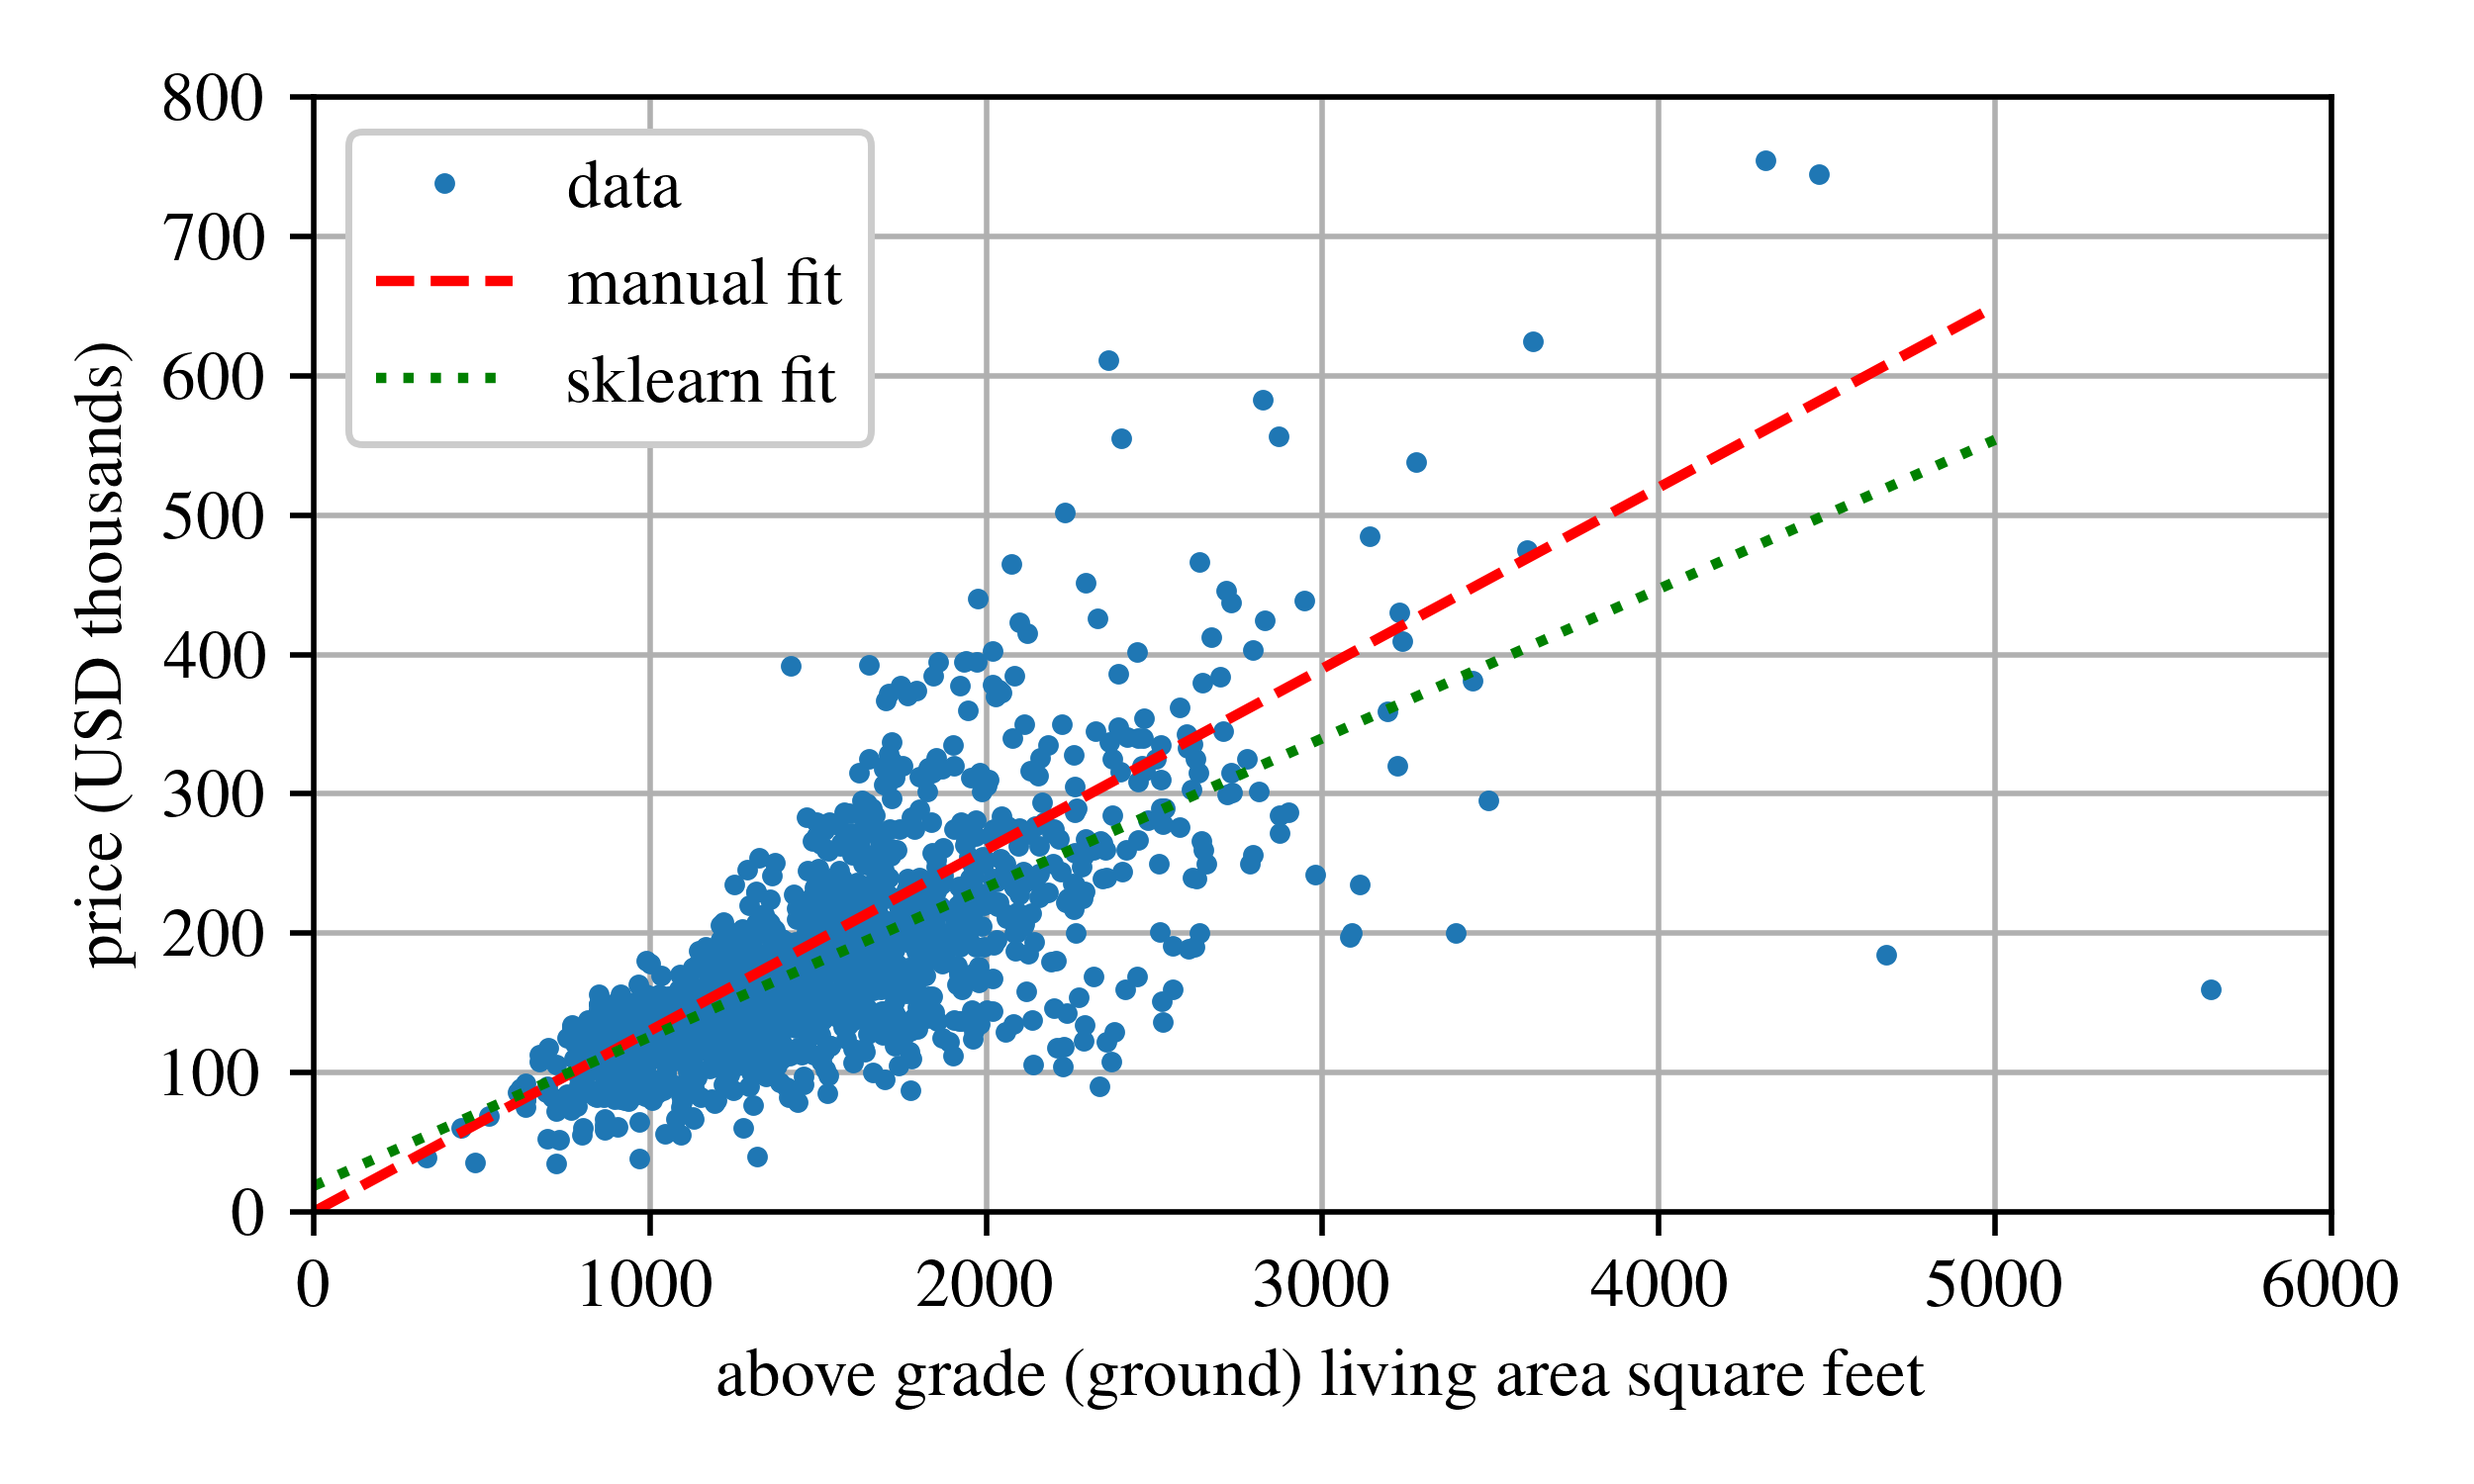
\includegraphics[width=\textwidth]{../figures/Ames_simple_linear_regression_model_2.png}
		\vspace{0.3em}
		{\small Ames housing data with trend lines.}
		\end{columns}
\end{frame}

%------------------------------------------------

\begin{frame}{Notation}
	\begin{center}
		\gr{Notations}
	\end{center}
\noindent In terms of linear algebra notation; we use:
\begin{itemize}
\item $\mathbf{x}$: lowercase bold symbols denote vectors.
\item $\mathbf{X}$: uppercase bold symbols denote matrices.
\end{itemize}	

In machine learning, we commonly use:
\begin{itemize}	
\item $\mathbf{X}$: the feature matrix (input data).
\item $\mathbf{y}$: the target vector (labels or outputs).
\item $\mathbf{x}^{(i)}$: the $i^\text{th}$ instance in the dataset.
\item $h$: the hypothesis or prediction function, $\hat{\mathbf{y}} = h(\mathbf{X})$.
\item $n$: the number of features.
\item $m$: the number of training instances.
\item $\hat{x}$: an estimated value (``$x$-hat'').
\end{itemize}
\end{frame}

%------------------------------------------------

\begin{frame}{Least Squares Intuition}
	\begin{columns}
		\column{0.48\textwidth}
		Goal:
		\begin{itemize}
			\item Find parameters that minimize error
			\item Fit a line closest to all data points
		\end{itemize}
		
		\vspace{0.5em}
		
		Idea:
		\begin{itemize}
			\item Measure vertical distance to line
			\item Square the errors
			\item Sum over all points
		\end{itemize}
		
		\column{0.52\textwidth}
		\centering
		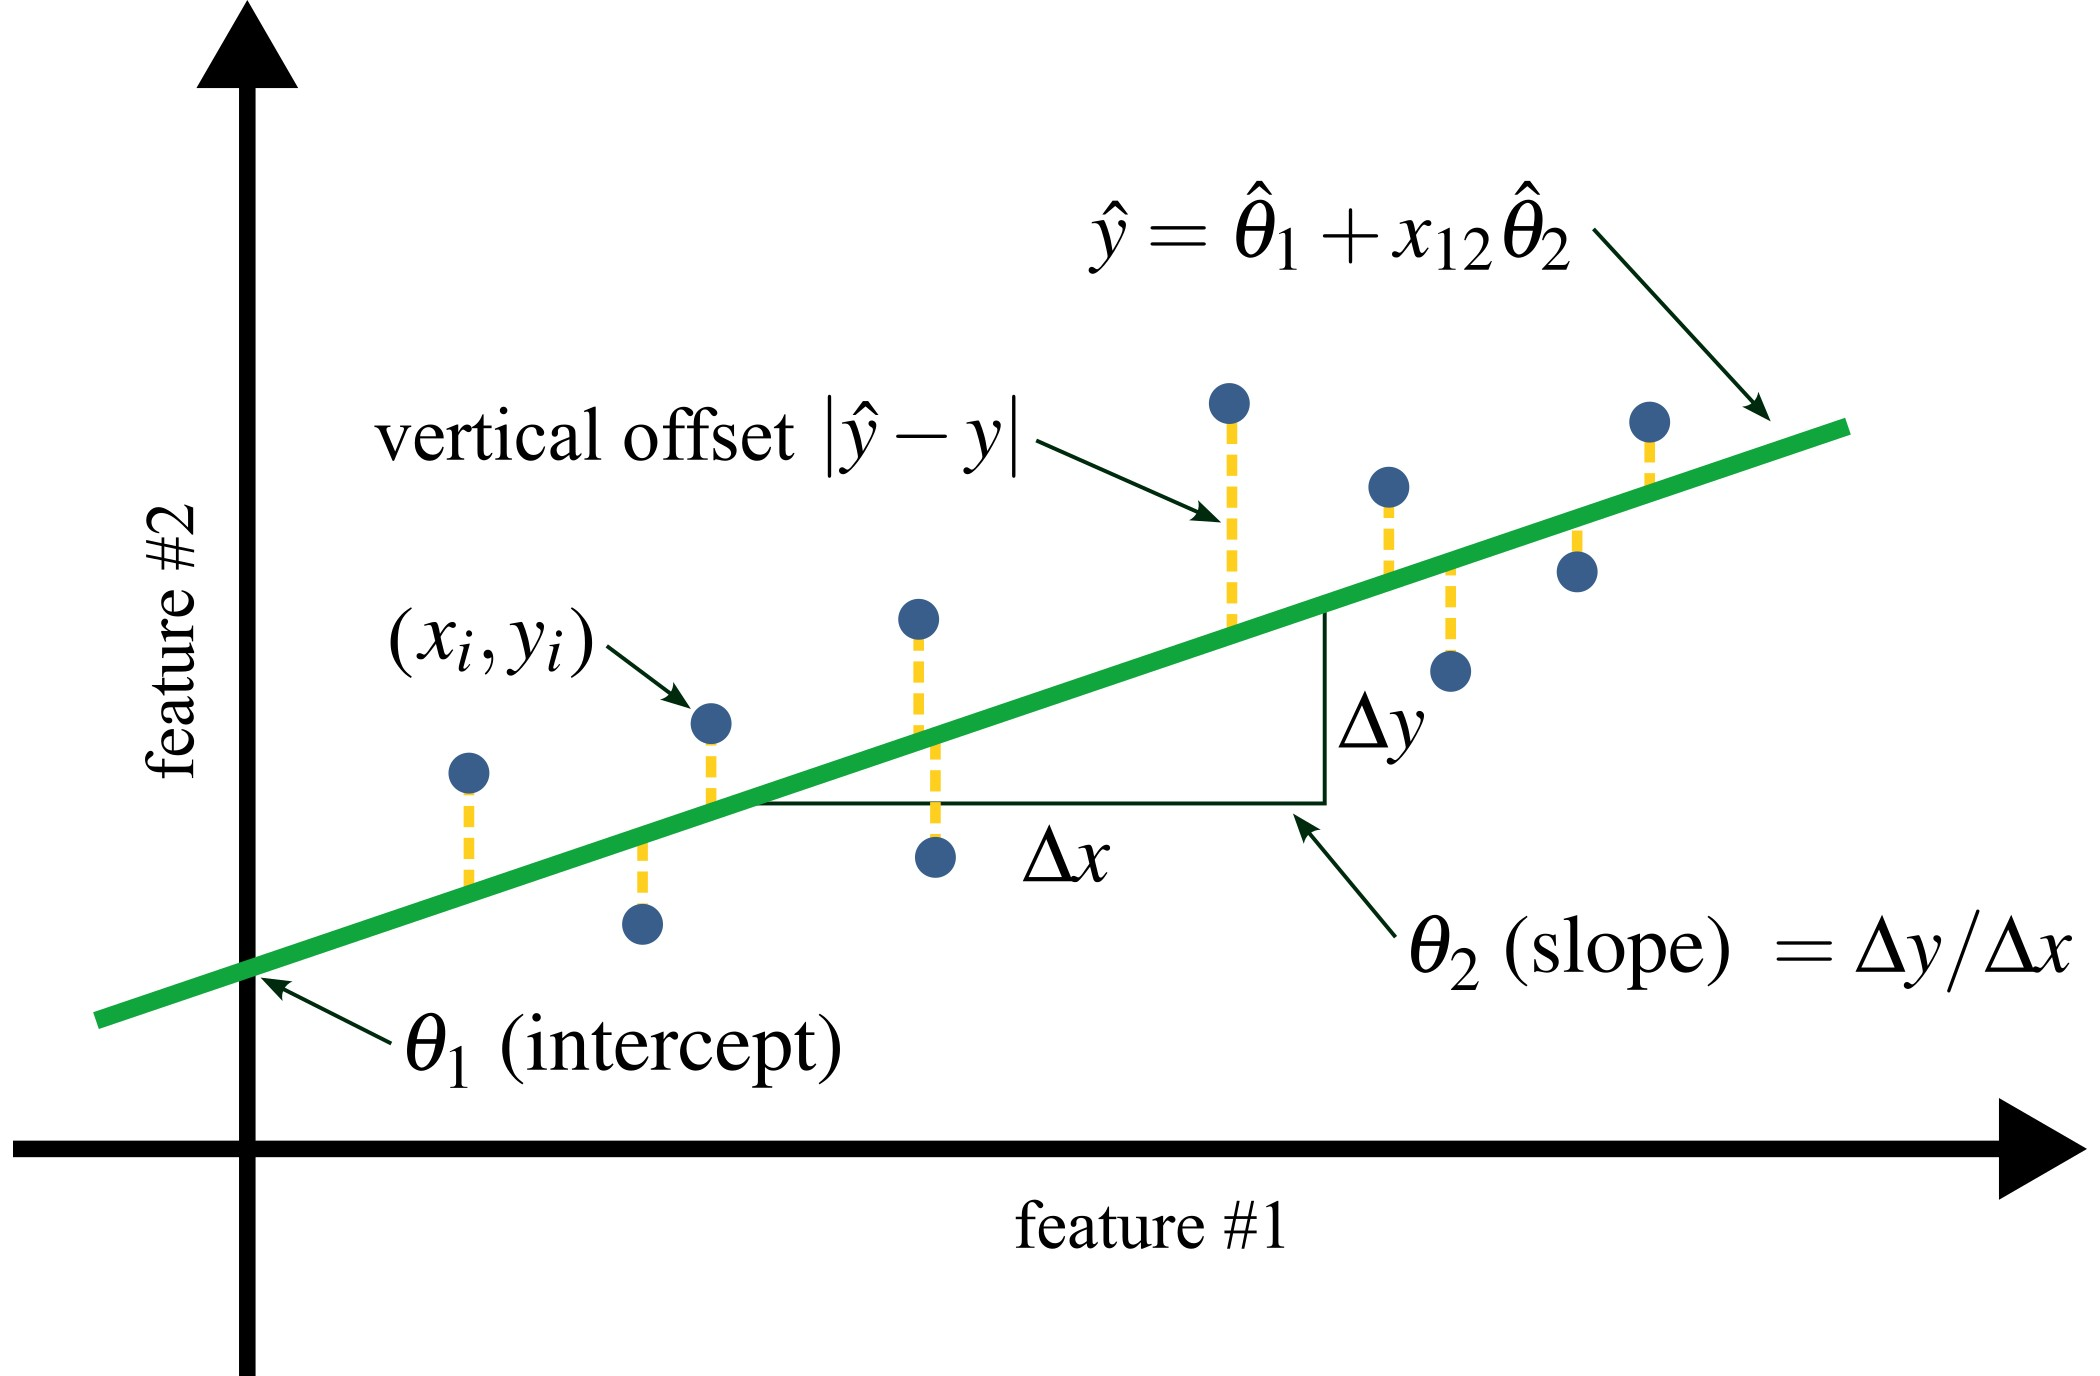
\includegraphics[width=\textwidth]{../figures/least_squares}
		
		\vspace{0.3em}
		{Least squares fit.}
		
	\end{columns}
\end{frame}

%------------------------------------------------

\begin{frame}{How Do We Measure Fit?}
	Before tuning a model, we need a way to measure how well it fits the data.
	\begin{itemize}
		\item Define a \textbf{cost function}
		\item Penalizes differences between predictions and true values
		\item Lower cost = better fit
	\end{itemize}
	\vspace{0.5em}
	For linear regression:
	\begin{itemize}
		\item Use \textbf{Ordinary Least Squares (OLS)}
		\item Minimizes prediction error over all training data
	\end{itemize}
\end{frame}

%------------------------------------------------

\begin{frame}{Mean Squared Error (MSE)}
	\small
	A common cost function is Mean Squared Error:
	\[
	J = \frac{1}{m} \sum_{i=1}^{m} (\hat{y}_i - y_i)^2
	\]
	\begin{itemize}
		\item $m$: number of data points
		\item Measures average squared prediction error
		\item Larger errors are penalized more heavily
	\end{itemize}
	\vspace{0.5em}
	For linear regression:
	\[
	J = \frac{1}{m} \sum_{i=1}^{m} (\bm{\theta}^{\top} \mathbf{x}^{(i)} - y^{(i)})^2
	\]
\end{frame}

%------------------------------------------------

\begin{frame}{Linear Regression Model}
	
	Consider a dataset with $n$ observations and $p$ features.
	
	\vspace{0.5em}
	
	For each observation:
	
	\[
	y_i =
	\theta_1 x_{i1} +
	\theta_2 x_{i2} +
	\cdots +
	\theta_p x_{ip} +
	\epsilon_i
	\]
	
	\vspace{0.5em}
	
	\begin{itemize}
		\item $y_i$: target value
		\item $x_{ij}$: feature values
		\item $\theta_j$: model parameters
		\item $\epsilon_i$: error term
	\end{itemize}
	
\end{frame}

%------------------------------------------------

\begin{frame}{Matrix Formulation}
	\begin{columns}
		
		\column{0.48\textwidth}
		
		We can write the linear model compactly:
		
		\[
		\mathbf{y} = \mathbf{X}\bm{\theta} + \epsilon
		\]
		
		\begin{itemize}
			\item $\mathbf{X}$: feature matrix
			\item $\bm{\theta}$: parameters
			\item $\mathbf{y}$: target values
		\end{itemize}
		
		\vspace{0.5em}
		
		Predictions:
		
		\[
		\hat{\mathbf{y}} = \mathbf{X}\hat{\bm{\theta}}
		\]
		
		\vspace{0.5em}
		
		Goal:
		\begin{itemize}
			\item Find $\hat{\bm{\theta}}$ that minimizes error
		\end{itemize}
		
		\column{0.52\textwidth}
		
		\[
		\mathbf{X} =
		\begin{bmatrix}
			x_{11} & x_{12} & \cdots & x_{1p} \\
			x_{21} & x_{22} & \cdots & x_{2p} \\
			\vdots & \vdots & \ddots & \vdots \\
			x_{n1} & x_{n2} & \cdots & x_{np}
		\end{bmatrix}
		\]
		
		\vspace{0.7em}
		
		\[
		\bm{\theta} =
		\begin{bmatrix}
			\theta_1 \\
			\theta_2 \\
			\vdots \\
			\theta_p
		\end{bmatrix}
		\qquad
		\mathbf{y} =
		\begin{bmatrix}
			y_1 \\
			y_2 \\
			\vdots \\
			y_n
		\end{bmatrix}
		\]
		
	\end{columns}
\end{frame}

%------------------------------------------------

\begin{frame}{The Normal Equation}
	\begin{columns}
		
		\column{0.48\textwidth}
		
		Closed-form solution:
		
		\[
		\hat{\bm{\theta}} = (\mathbf{X}^{\top} \mathbf{X})^{-1} \mathbf{X}^{\top} \mathbf{y}
		\]
		
		\begin{itemize}
			\item Gives the exact best-fit parameters
			\item No iteration required
			\item Works well for small feature sets
		\end{itemize}
		
		\vspace{0.5em}
		
		For a simple model:
		
		\[
		\hat{y} = \hat{\theta}_1 + x \hat{\theta}_2
		\]
		
		This is just:
		
		\[
		y = mx + b
		\]
		
		\column{0.52\textwidth}
		\centering
		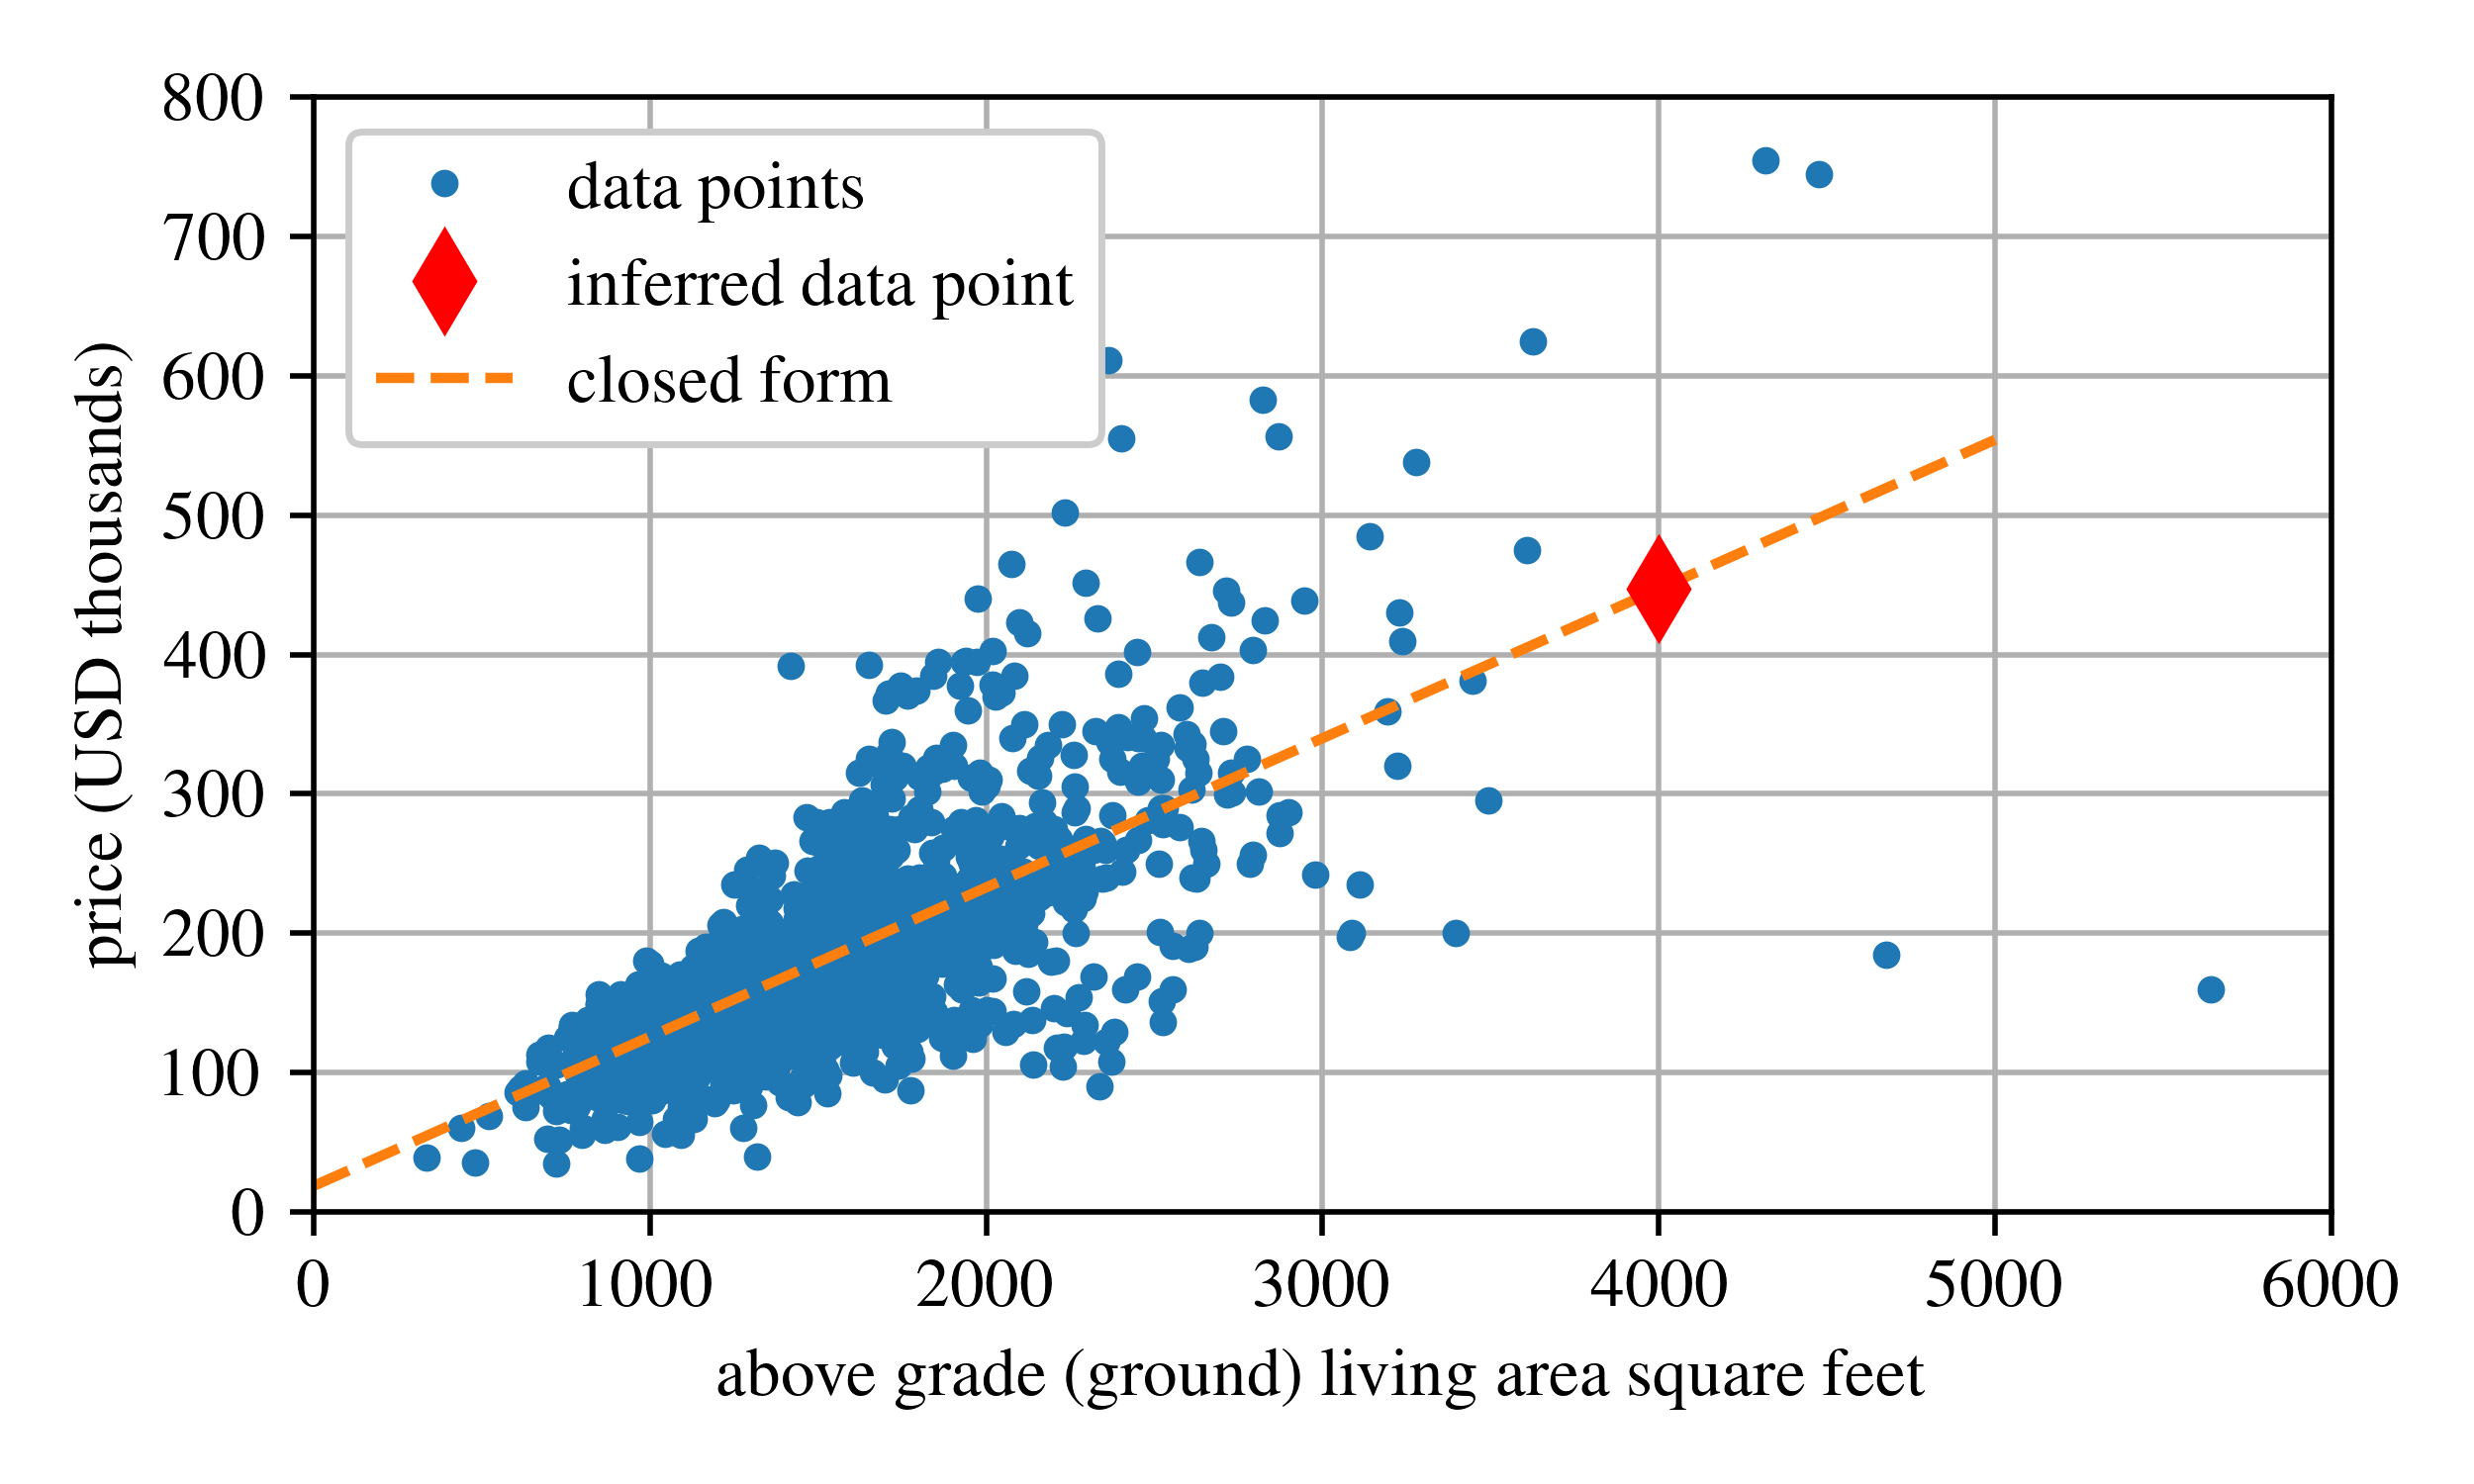
\includegraphics[width=\textwidth]{../figures/Ames_simple_linear_regression_model_3.png}
		
		\vspace{0.3em}
		{\small Ames housing data inferred.}
		
	\end{columns}
\end{frame}

%------------------------------------------------

\begin{frame}{Computational Complexity}
	\begin{itemize}
		\item Normal Equation requires inverting $\mathbf{X}^{\top}\mathbf{X}$ (an $n \times n$ matrix)
		\item Matrix inversion cost: $O(n^{2.4})$ to $O(n^3)$
		\item Doubling features $\Rightarrow$ $\sim 5$--$8\times$ more computation
	\end{itemize}
	
	\begin{alertblock}{Warning}
		For very large feature sets (e.g., $n \sim 100{,}000$), the Normal Equation becomes extremely slow.
	\end{alertblock}
	
	\begin{itemize}
		\item Scales linearly with number of instances: $O(m)$
		\item Prediction is fast: linear in both $m$ and $n$
	\end{itemize}
\end{frame}

%------------------------------------------------

\begin{frame}{Example 2.1: Ames Housing (Linear Regression)}
	\begin{itemize}
		\item Fit a linear model to predict house price from living area
		\item Compare approaches:
		\begin{itemize}
			\item Manual fit (visual intuition)
			\item Closed-form (Normal Equation)
			\item Gradient Descent
		\end{itemize}
		\item In practice (scikit-learn):
		\begin{itemize}
			\item \texttt{LinearRegression} (closed-form)
			\item \texttt{SGDRegressor} (iterative)
		\end{itemize}
	\end{itemize}
	
	\vspace{0.5em}
	Next: methods that scale better for large feature sets or large datasets.
\end{frame}

%------------------------------------------------

\section{2.2~Gradient Descent}

\begin{frame}{Gradient Descent}
	\begin{columns}
		
		\column{0.48\textwidth}
		
		\begin{itemize}
			\item Optimization algorithm to minimize a cost function
			\item Iteratively updates parameters
		\end{itemize}
		
		\vspace{0.5em}
		
		Idea:
		\begin{enumerate}
			\item Compute the gradient (slope)
			\item Move in direction of steepest descent
			\item Repeat until minimum is reached
		\end{enumerate}
		
		\column{0.52\textwidth}
		\centering
		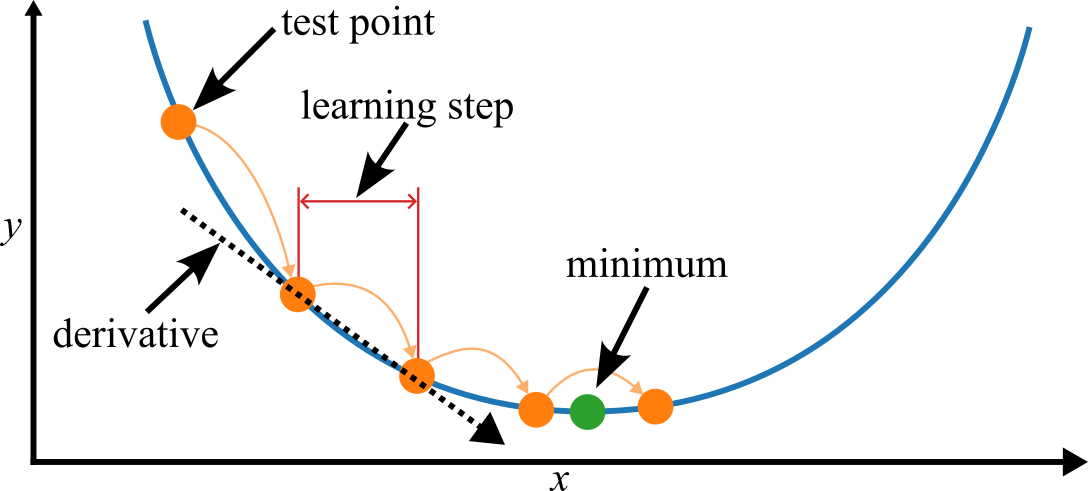
\includegraphics[width=\textwidth]{../figures/gradient_descent_1}
		
		\vspace{0.3em}
		{\small Gradient descent moving toward a minimum.}
		
	\end{columns}
\end{frame}

%------------------------------------------------

\begin{frame}{Learning Rate}
	\begin{columns}
		
		\column{0.48\textwidth}
		
		\begin{itemize}
			\item Step size controlled by learning rate $\eta$
		\end{itemize}
		
		\vspace{0.5em}
		
		\begin{itemize}
			\item Small $\eta$ $\rightarrow$ slow convergence
			\item Large $\eta$ $\rightarrow$ overshooting / divergence
		\end{itemize}
		
		\vspace{0.5em}
		
		Choosing $\eta$ is critical
		
		\column{0.52\textwidth}
		\centering
		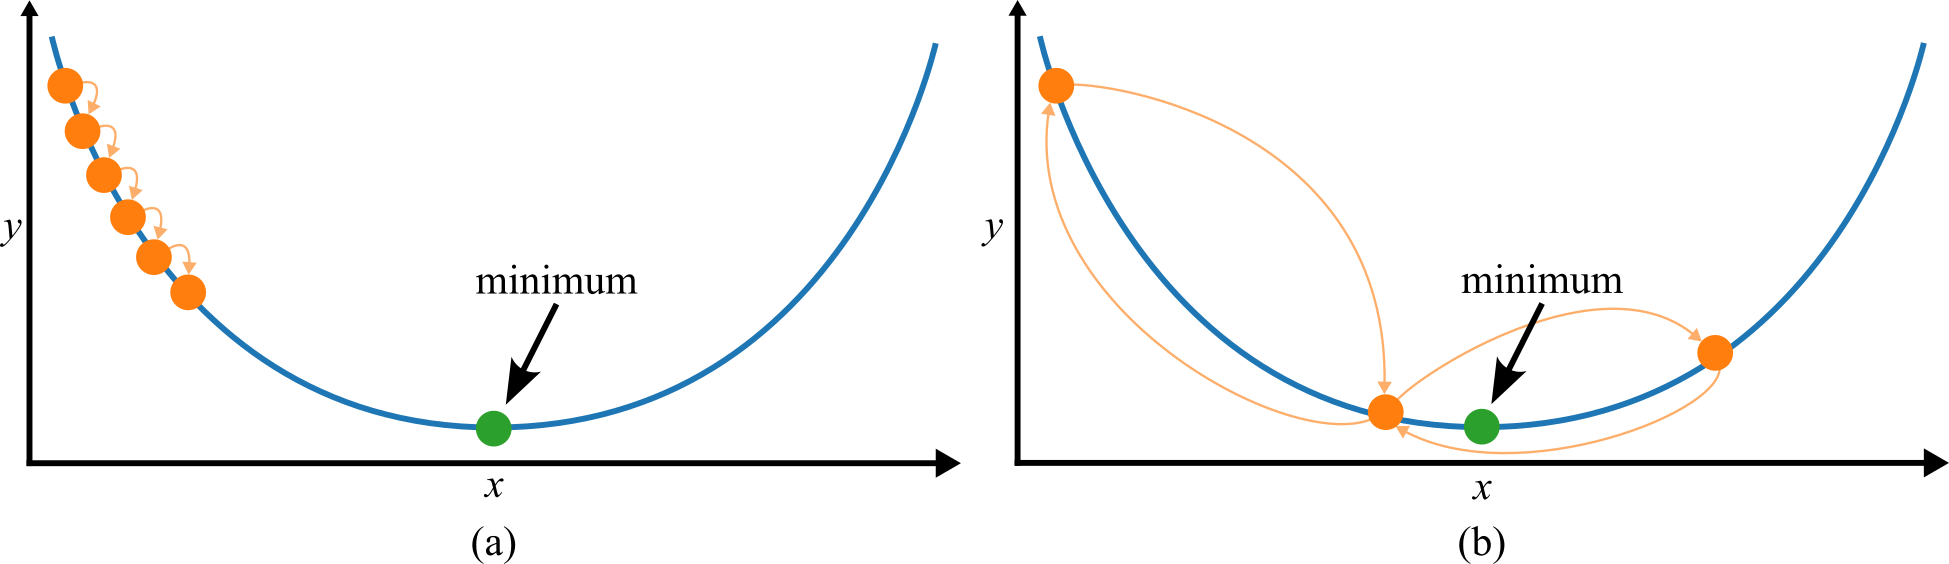
\includegraphics[width=0.75\textwidth,trim=0cm 0cm 3.3in 0cm,clip]{../figures/gradient_descent_2}
		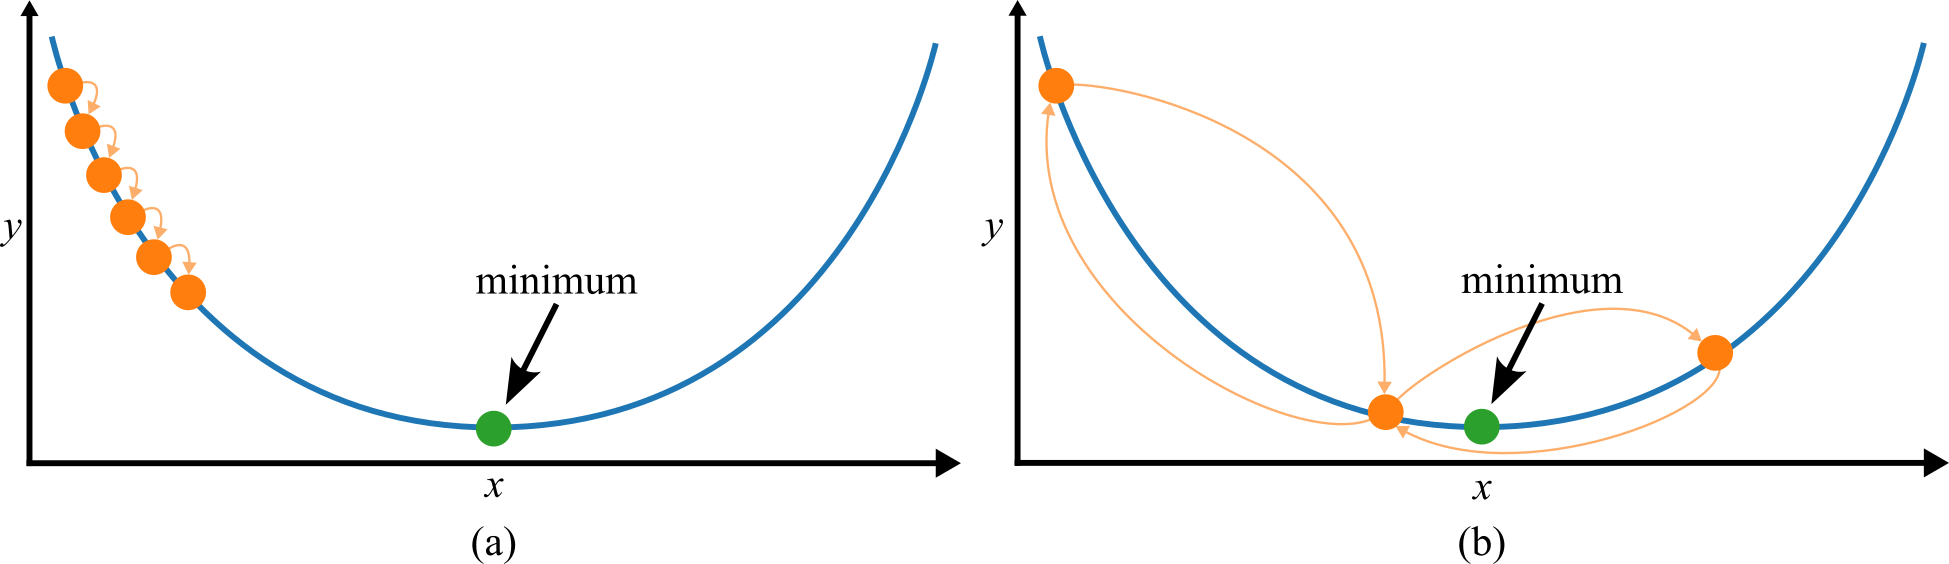
\includegraphics[width=0.75\textwidth,trim=3.30in 0cm 0cm 0cm,clip]{../figures/gradient_descent_2}
		
		\vspace{0.3em}
		{\small Effect of different learning rates.}
		
	\end{columns}
\end{frame}

%------------------------------------------------

\begin{frame}{Challenges}
	\begin{columns}
		
		\column{0.48\textwidth}
		
		\begin{itemize}
			\item Cost functions may be complex:
			\begin{itemize}
				\item Local minima
				\item Plateaus
				\item Ridges
			\end{itemize}
			
			\vspace{0.5em}
			
			\item Starting point matters
			\item Convergence may be slow
		\end{itemize}
		
		\vspace{0.5em}
		
		For linear regression:
		\begin{itemize}
			\item MSE is convex
			\item One global minimum
		\end{itemize}
		
		\column{0.52\textwidth}
		\centering
		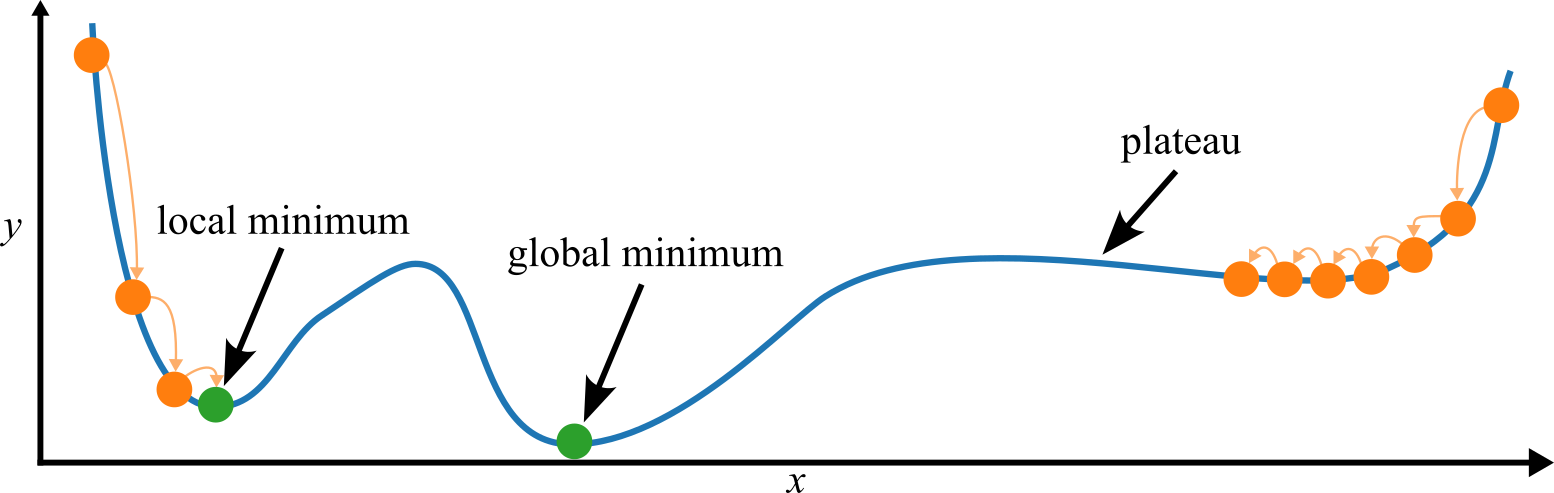
\includegraphics[width=\textwidth]{../figures/gradient_descent_3}
		
		\vspace{0.3em}
		{\small Optimization challenges in complex landscapes.}
		
	\end{columns}
\end{frame}

%------------------------------------------------

\begin{frame}{Comparing Gradient Descent Methods}
	\begin{columns}
		
		\column{0.48\textwidth}
		
		\begin{itemize}
			\item Different methods reach the minimum differently
			\item Trade-off between speed and stability
			\item Some methods are noisy but fast
			\item Others are stable but computationally expensive
		\end{itemize}
		
		\vspace{0.5em}
		
		All aim to minimize the same cost function
		
		\column{0.52\textwidth}
		\centering
		
\includegraphics[width=\textwidth]{../figures/comparing_gradient_descent_methods}
		
		\vspace{0.3em}
		{\small Paths taken by different methods.}
		
	\end{columns}
\end{frame}

%------------------------------------------------

\begin{frame}{Method Comparison}
	Different approaches to linear regression vary in speed, scalability, and flexibility.
	\vspace{0.5em}
	
	\centering
	\resizebox{\textwidth}{!}{
		\begin{tabular}{lllllll}
			\toprule
			algorithm & large $m$ & in memory & large $n$ & hyperparams & scaling & sklearn \\ \midrule
			normal equation & fast & yes & slow & 0 & no & \texttt{LinearRegression} \\
			batch GD & slow & yes & fast & 2 & yes & n/a \\
			stochastic GD & fast & no & fast & $\ge 2$ & yes & \texttt{SGDRegressor} \\
			mini-batch GD & fast & no & fast & $\ge 2$ & yes & n/a \\ \bottomrule
		\end{tabular}
	}
	
	\vspace{0.5em}
	
\begin{mdframed}[middlelinewidth=0.5mm]
	\begin{center}
		\bl{NOTE}
	\end{center}
	After training, there is minimal difference between the models: these algorithms converge on similar solutions and make predictions in a nearly identical manner.
\end{mdframed}

\end{frame}

%------------------------------------------------

\begin{frame}{Batch Gradient Descent}
	\begin{columns}
		
		\column{0.48\textwidth}
		
		\begin{itemize}
			\item Uses the entire dataset at each step
			\item Minimizes the cost function over all data
			\item Based on Mean Squared Error (MSE)
		\end{itemize}
		
		\vspace{0.5em}
		
		\[
		J = \frac{1}{m} \sum_{i=1}^{m} (\bm{\theta}^{\top}\mathbf{x}^{(i)} - y^{(i)})^2
		\]
		
		\vspace{0.5em}
		
		\begin{itemize}
			\item Computes exact gradient each iteration
			\item Can be slow for large datasets
		\end{itemize}
		
		\column{0.52\textwidth}
		\centering
		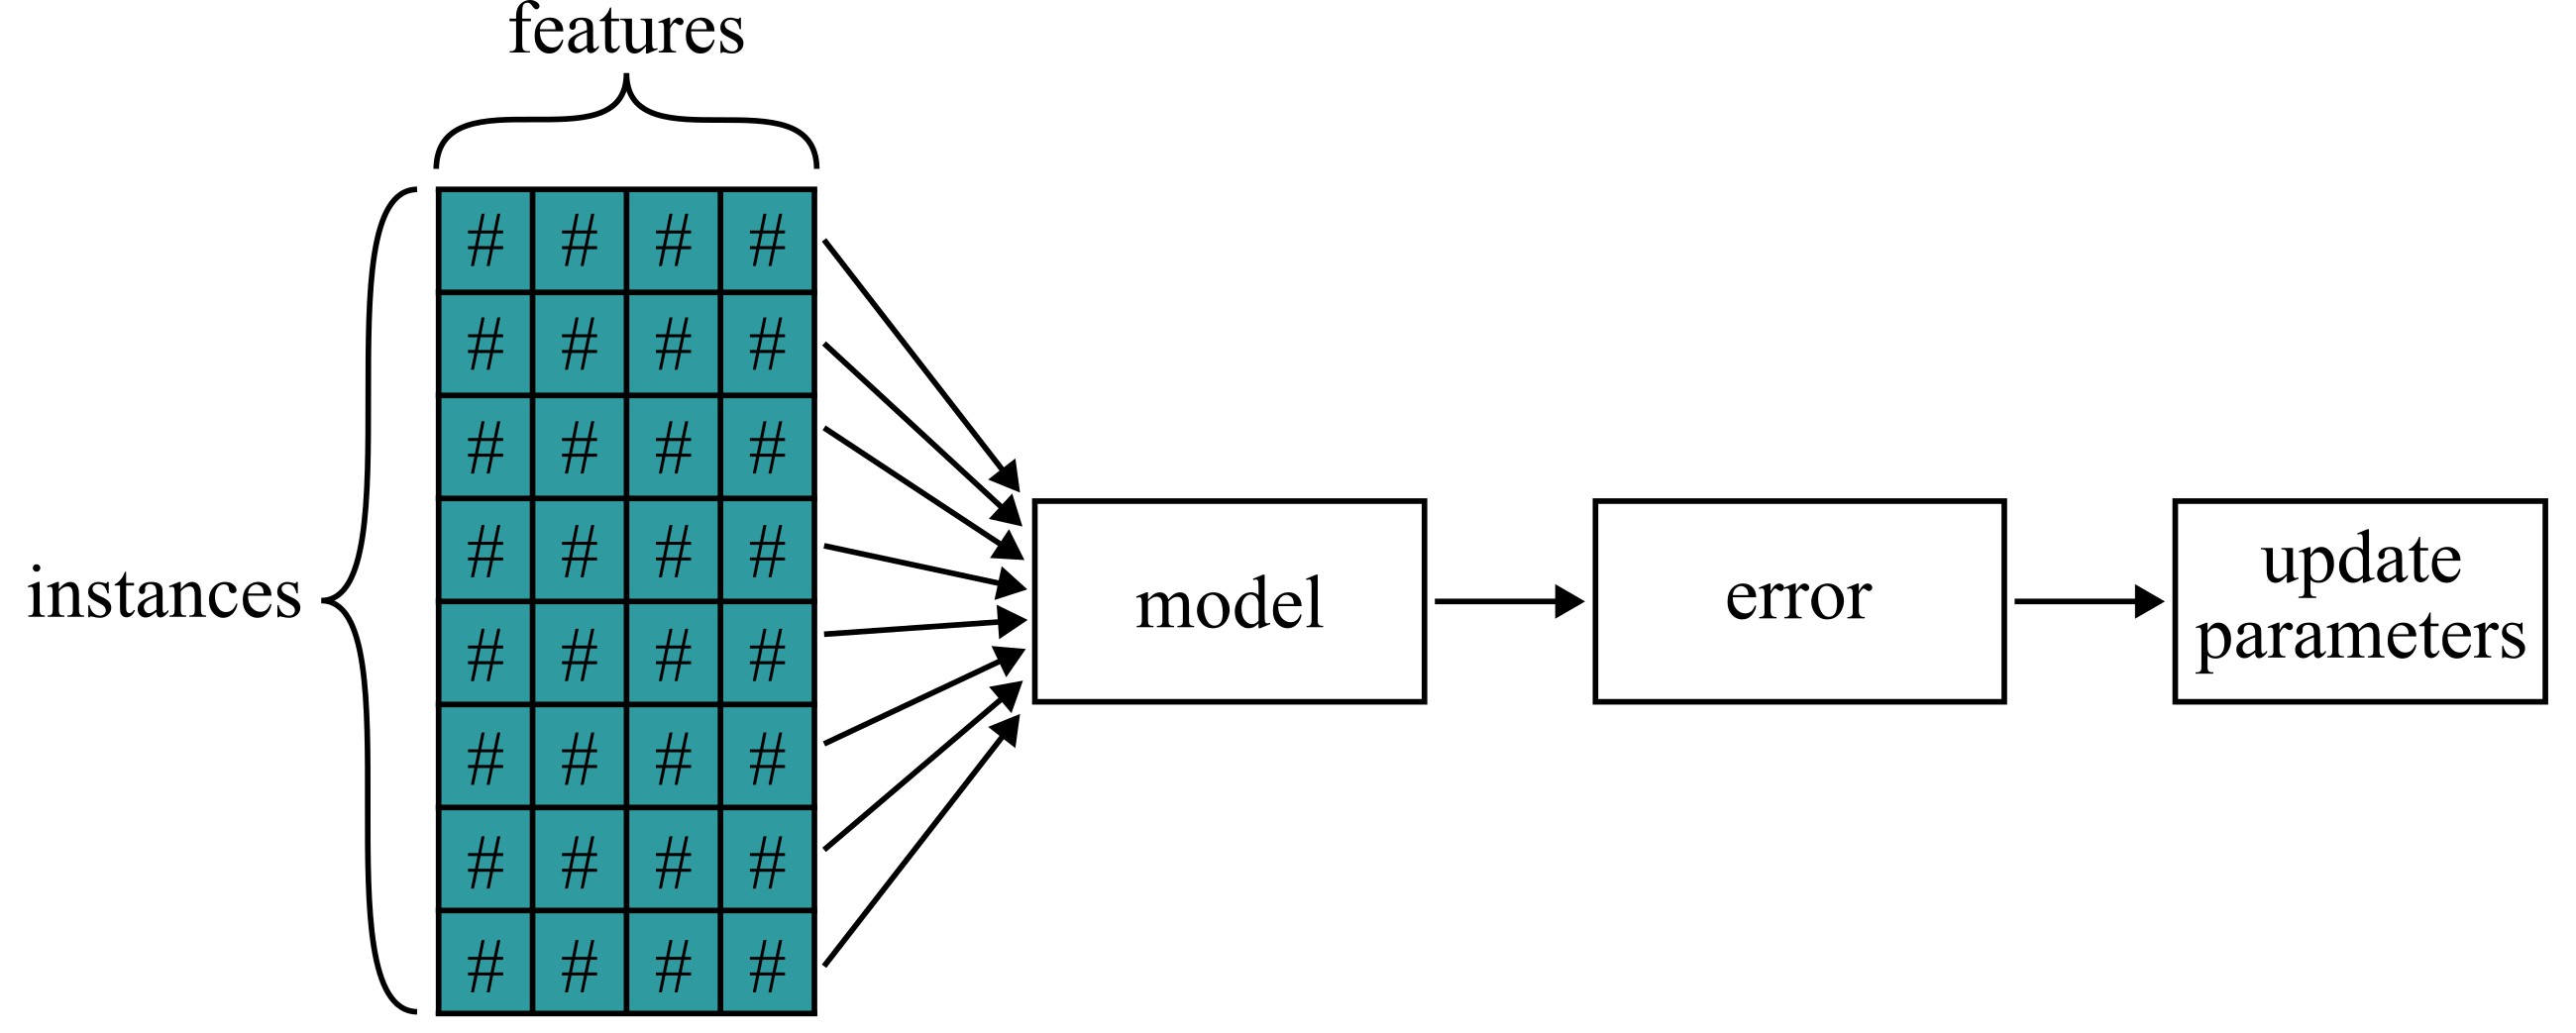
\includegraphics[width=\textwidth]{../figures/gradient_descent_batch}
		
		\vspace{0.3em}
		{\small Batch Gradient Descent flow.}
		
	\end{columns}
\end{frame}

%------------------------------------------------

\begin{frame}{Gradient Computation}
	\begin{columns}
		
		\column{0.48\textwidth}
		
		Compute partial derivatives:
		
		\[
		\frac{\partial}{\partial \theta_j} J(\theta) =
		\frac{2}{m} \sum_{i=1}^{m}
		(\bm{\theta}^{\top}\mathbf{x}^{(i)} - y^{(i)}) x_j^{(i)}
		\]
		
		\vspace{0.5em}
		
		Vector form:
		
		\[
		\nabla_\theta J(\bm{\theta}) =
		\frac{2}{m}\mathbf{X}^{\top}(\mathbf{X}\bm{\theta} - \mathbf{y})
		\]
		
		\vspace{0.5em}
		
		\begin{itemize}
			\item Computes all slopes at once
			\item Direction of steepest ascent
		\end{itemize}
		
		\column{0.52\textwidth}
		
		\begin{exampleblock}{Key Idea}
			Move in the opposite direction of the gradient to reduce error.
		\end{exampleblock}
		
		\vspace{0.5em}
		
		\begin{alertblock}{Warning}
			Uses the full dataset at every step → can be slow for large $m$.
		\end{alertblock}
		
	\end{columns}
\end{frame}

%------------------------------------------------

\begin{frame}{Parameter Update and Learning Rate}
	\begin{columns}
		
		\column{0.48\textwidth}
		
		Update rule:
		
		\[
		\bm{\theta}^{(\text{next})}
		= \bm{\theta} - \eta \nabla_\theta J(\bm{\theta})
		\]
		
		\vspace{0.5em}
		
		\begin{itemize}
			\item $\eta$: learning rate (step size)
			\item Controls speed of convergence
		\end{itemize}
		
		\vspace{0.5em}
		
		\begin{itemize}
			\item Too large → divergence
			\item Too small → slow convergence
			\item Just right → fast convergence
		\end{itemize}
		
		\column{0.52\textwidth}
		\centering
		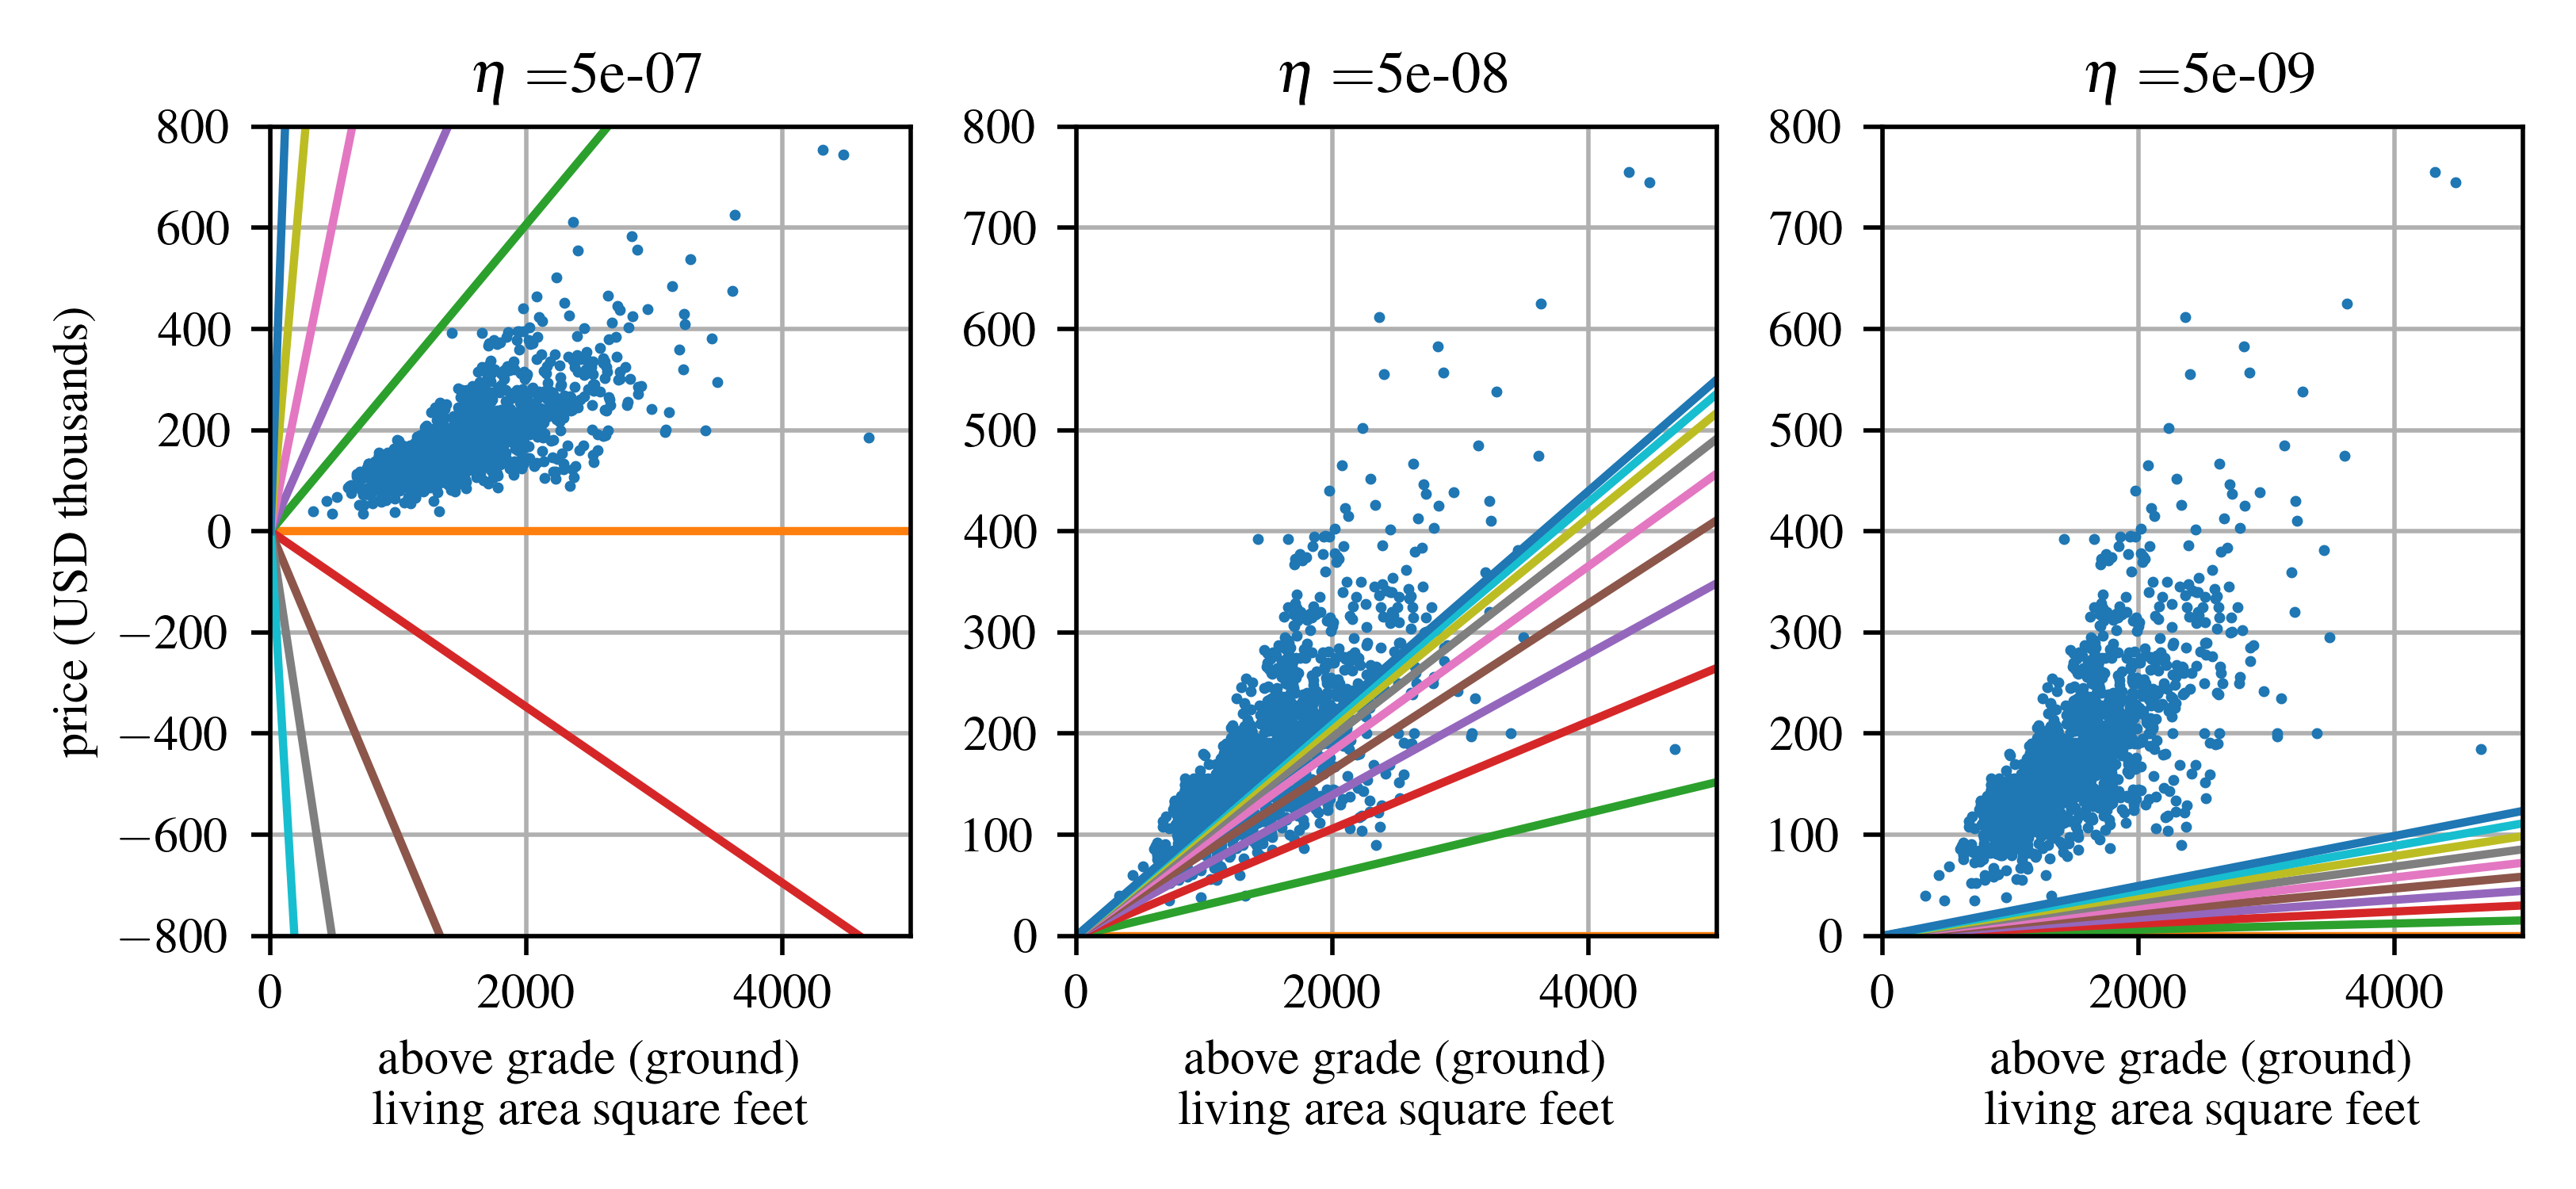
\includegraphics[width=\textwidth]{../figures/Ames_learning_rates.png}
		
		\vspace{0.3em}
		{\small Effect of different learning rates.}
		
	\end{columns}
\end{frame}

%------------------------------------------------



\begin{frame}{Stochastic Gradient Descent}
	\begin{columns}
		
		\column{0.48\textwidth}
		
		\begin{itemize}
			\item Updates parameters using one sample at a time
			\item Uses $(x^{(i)}, y^{(i)})$ instead of full dataset
		\end{itemize}
		
		\vspace{0.5em}
		
		\begin{itemize}
			\item Faster for large datasets
			\item Enables online learning
		\end{itemize}
		
		\column{0.52\textwidth}
		\centering
		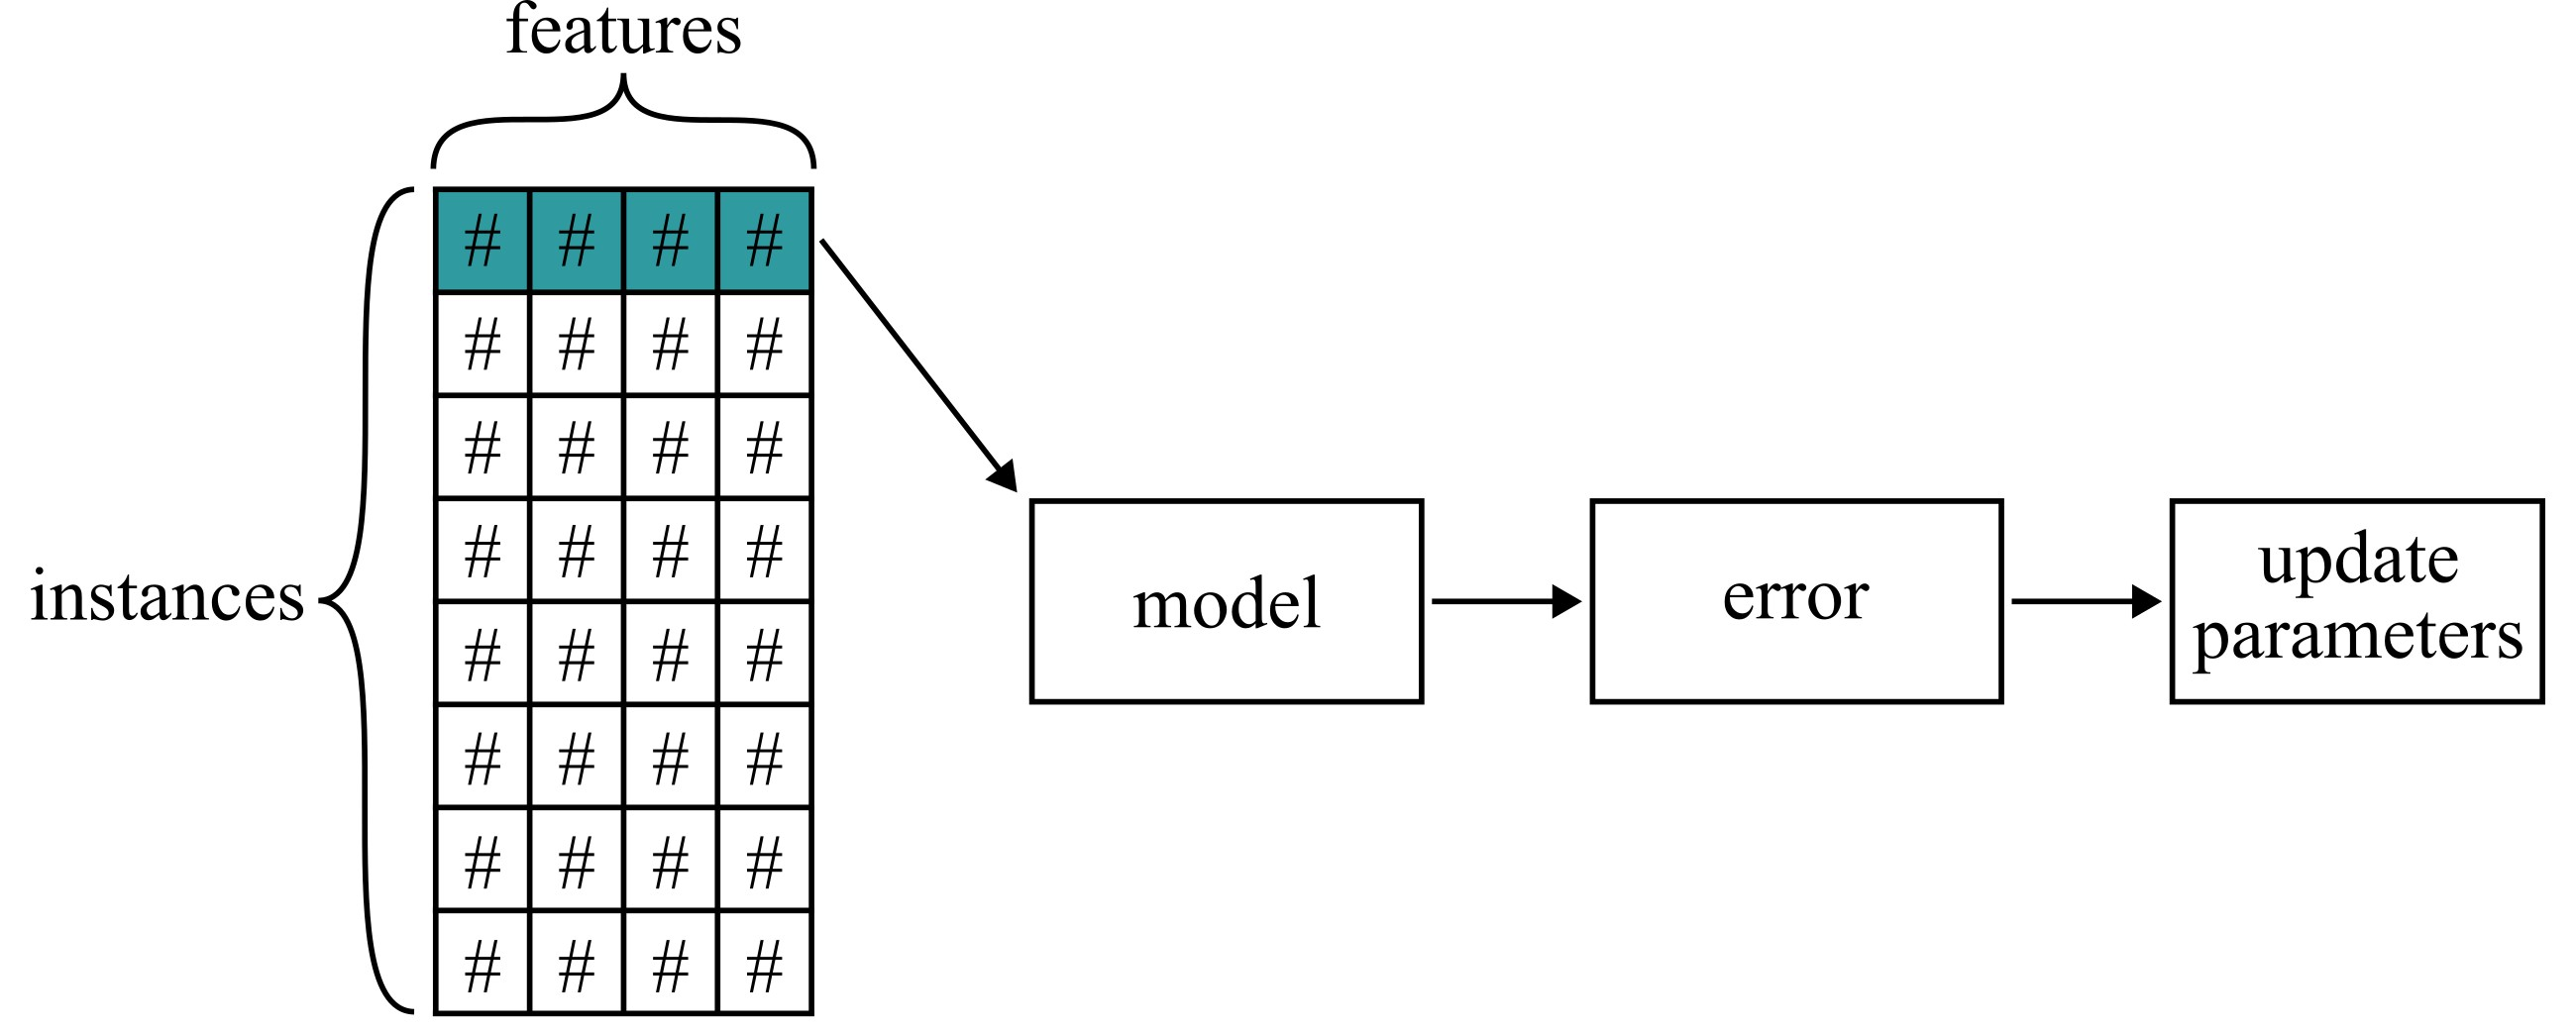
\includegraphics[width=\textwidth]{../figures/gradient_descent_stochastic}
		
		\vspace{0.3em}
		{\small Flow of Stochastic Gradient Descent.}
		
	\end{columns}
\end{frame}

%------------------------------------------------

\begin{frame}{SGD Update Rule}
	\begin{columns}
		
		\column{0.48\textwidth}
		
		Update rule:
		
		\[
		\bm{\theta}^{(\text{next})}
		= \bm{\theta} - \eta \nabla_\theta J(\bm{\theta}; x^{(i)}, y^{(i)})
		\]
		
		\vspace{0.5em}
		
		\begin{itemize}
			\item Updates after every single example
			\item Avoids redundant computations
			\item More efficient than Batch GD for large $m$
		\end{itemize}
		
		\column{0.52\textwidth}
		
		\begin{exampleblock}{Key Idea}
			Instead of waiting to see all data, update immediately using each new sample.
		\end{exampleblock}
		
	\end{columns}
\end{frame}

%------------------------------------------------

\begin{frame}{SGD Behavior}
	\begin{columns}
		
		\column{0.48\textwidth}
		
		\begin{itemize}
			\item Fast updates, but noisy path
			\item High variance in cost function
			\item Does not decrease smoothly
		\end{itemize}
		
		\vspace{0.5em}
		
		\begin{itemize}
			\item Often oscillates around minimum
			\item Can still reach a good solution
		\end{itemize}
		
		\column{0.52\textwidth}
		\centering
		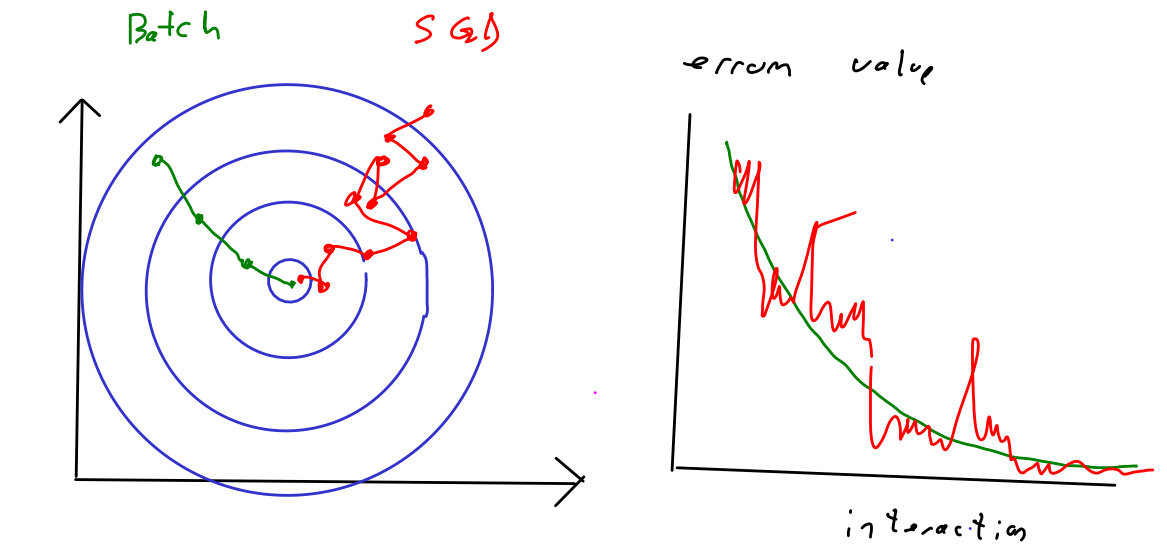
\includegraphics[width=\textwidth]{../figures/stochastic_gradient_descent_target}
		
		\vspace{0.3em}
		{\small Batch vs. stochastic gradient descent behavior.}
		
	\end{columns}
\end{frame}

%------------------------------------------------

\begin{frame}{Mini-batch Gradient Descent}
	\begin{columns}
		
		\column{0.48\textwidth}
		
		\begin{itemize}
			\item Uses small random subsets (mini-batches)
			\item Between Batch GD and Stochastic GD
		\end{itemize}
		
		\vspace{0.5em}
		
		Update rule:
		
		\[
		\bm{\theta}^{(\text{next})}
		= \bm{\theta} - \eta \nabla_\theta J(\bm{\theta}; x^{(i:i+n)}, y^{(i:i+n)})
		\]
		
		\vspace{0.5em}
		
		\begin{itemize}
			\item Faster than Batch GD
			\item More stable than SGD
			\item Efficient on GPUs (matrix operations)
		\end{itemize}
		
		\column{0.52\textwidth}
		\centering
		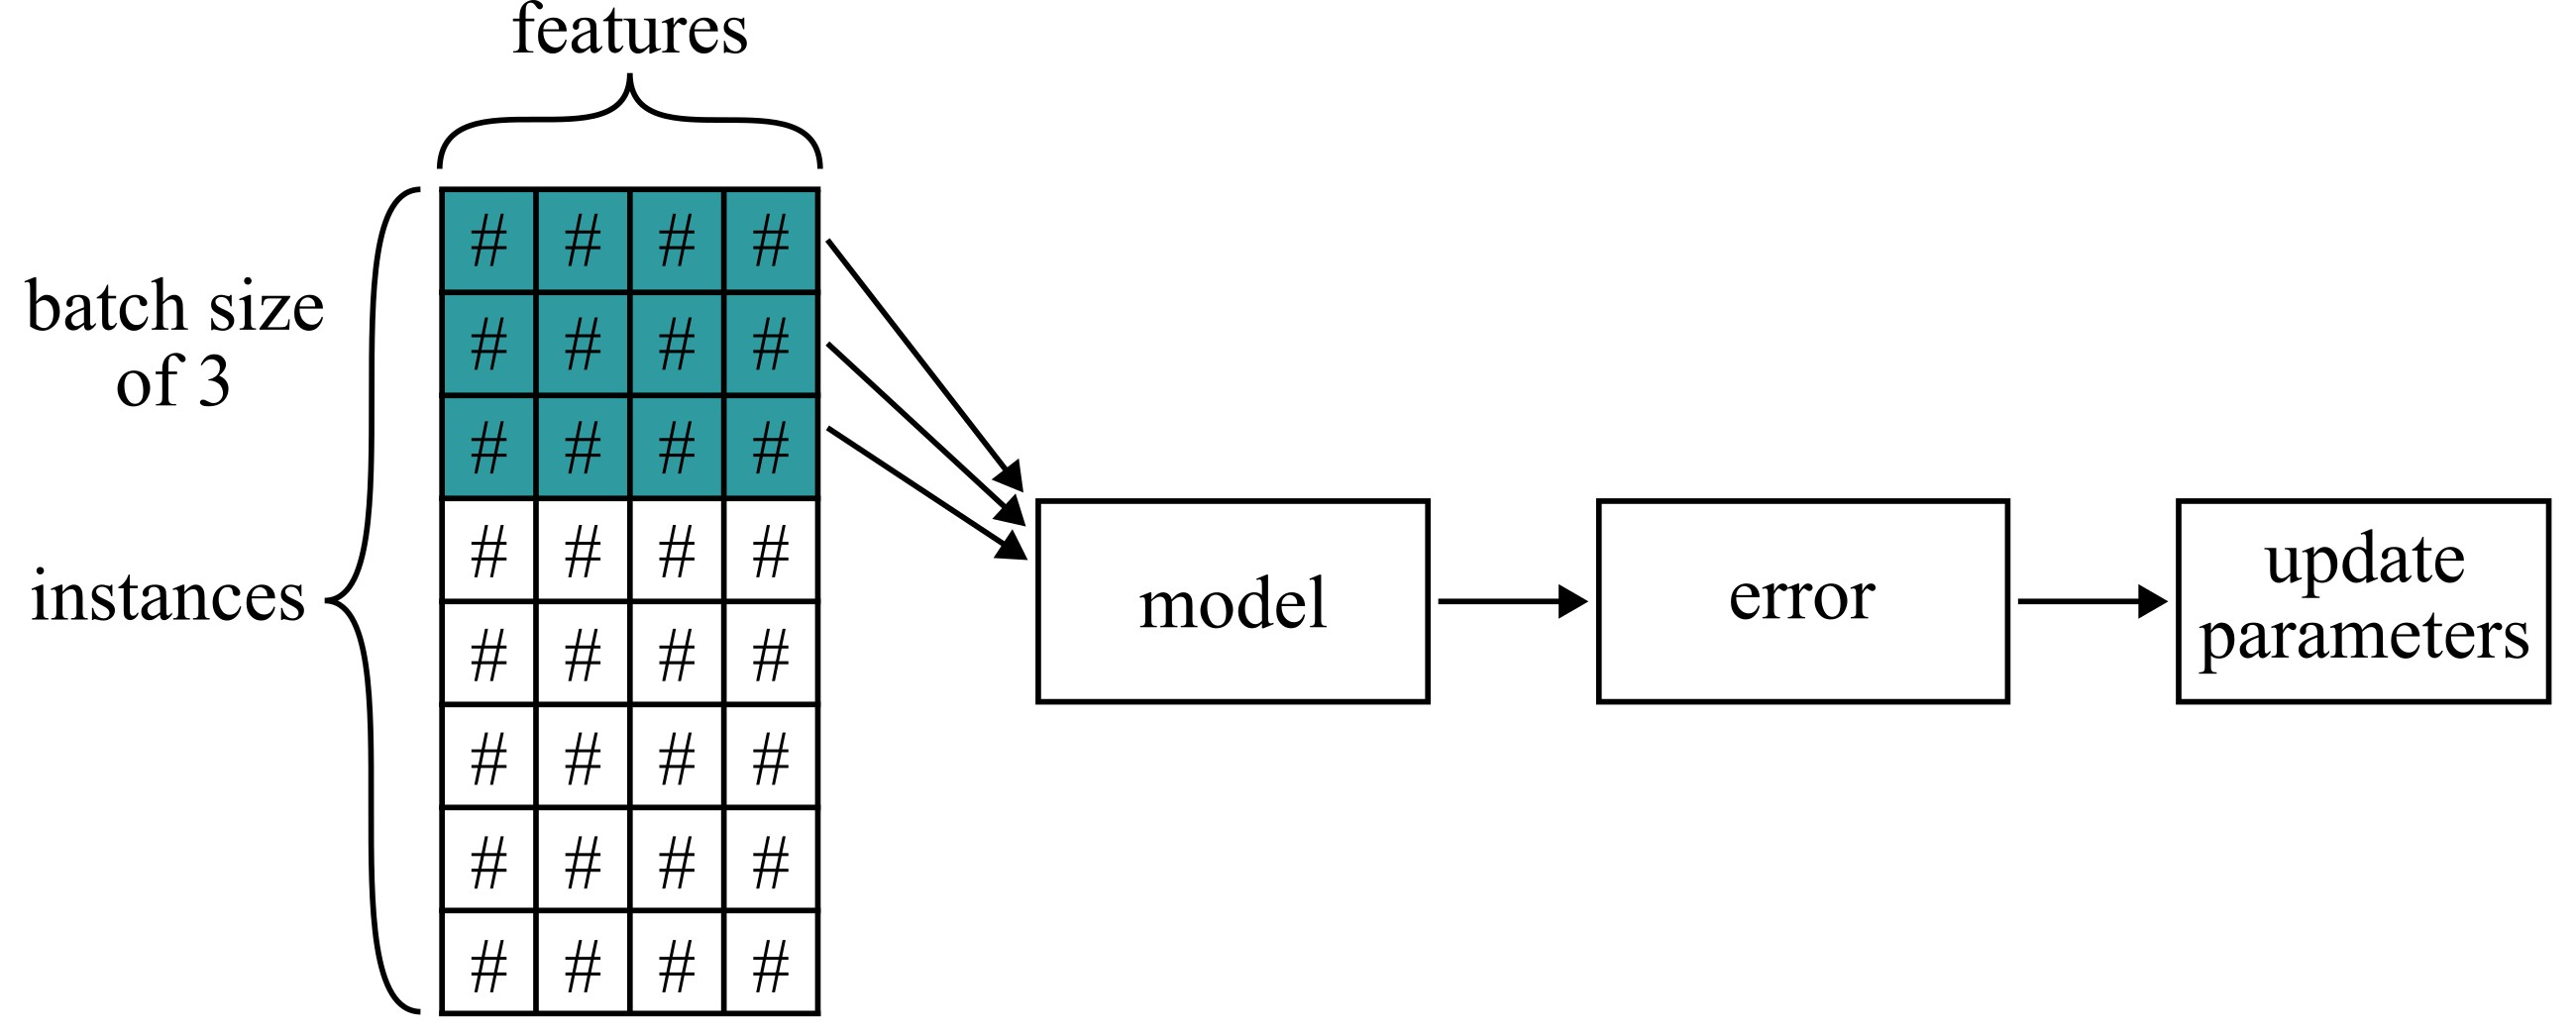
\includegraphics[width=\textwidth]{../figures/gradient_descent_mini_batch}
		
		\vspace{0.3em}
		{\small Flow of Mini-batch Gradient Descent.}
		
	\end{columns}
\end{frame}

%------------------------------------------------

\section{2.3~Feature Scaling}

\begin{frame}{Feature Scaling}
	\begin{columns}
		
		\column{0.48\textwidth}
		
		\begin{itemize}
			\item Different feature scales distort the cost surface
			\item Creates an elongated “valley”
		\end{itemize}
		
		\vspace{0.5em}
		
		\begin{itemize}
			\item Equal scaling $\rightarrow$ fast convergence
			\item Unequal scaling $\rightarrow$ slow convergence
		\end{itemize}
		
		\vspace{0.5em}
		
		Gradient Descent becomes inefficient without scaling
		
		\column{0.52\textwidth}
		\centering
		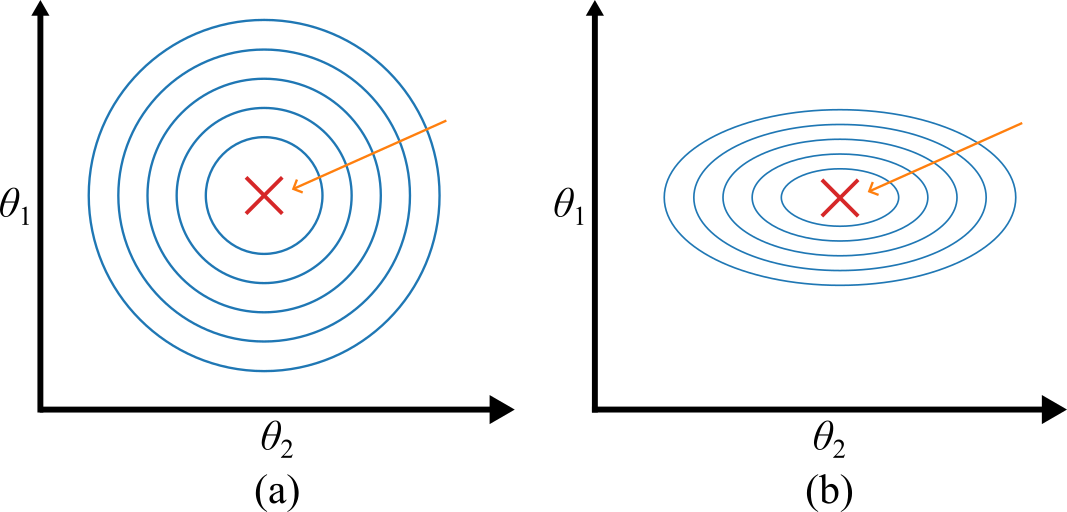
\includegraphics[width=\textwidth]{../figures/gradient_descent_5.png}
		
		\vspace{0.3em}
		{\small Effect of feature scaling on convergence.}
		
	\end{columns}
\end{frame}

%------------------------------------------------

\begin{frame}{Scaling Methods}
	\begin{columns}
		
		\column{0.48\textwidth}
		
		\textbf{Min-max scaling}
		\[
		\mathbf{X}' =
		\frac{\mathbf{X} - \mathbf{X}_{\min}}
		{\mathbf{X}_{\max} - \mathbf{X}_{\min}}
		\]
		
		\begin{itemize}
			\item Rescales to $[0,1]$
			\item Sensitive to outliers
		\end{itemize}
		
		\vspace{0.5em}
		
		\textbf{Standardization}
		\[
		\mathbf{X}' =
		\frac{\mathbf{X} - \overline{\mathbf{X}}}{\sigma}
		\]
		
		\begin{itemize}
			\item Zero mean, unit variance
			\item Less sensitive to outliers
		\end{itemize}
		
		\column{0.52\textwidth}
		
		\begin{itemize}
			\item Both improve Gradient Descent performance
			\item Standardization is most commonly used
		\end{itemize}
		
		\vspace{0.5em}
		
		\begin{exampleblock}{Tools}
			\texttt{MinMaxScaler} \\
			\texttt{StandardScaler}
		\end{exampleblock}
		
	\end{columns}
\end{frame}








































































\end{document}




